\documentclass{llncs}

%%%%%%%%%%%%%%%%%%%%%%%%%%%%%%%%%%%%%%%%%%%%% General %%%%%%%%%%%%%%%%%%%%%%%%%%%%%%%%%%%%%%%%%%%%%%
\usepackage[dvipsnames]{xcolor}
\usepackage{array}
\usepackage{nameref}
\usepackage{acronym}
\usepackage{diagbox}
\usepackage{enumitem}
\usepackage{multirow}
\usepackage{booktabs}
\usepackage{makecell}

%%%%%%%%%%%%%%%%%%%%%%%%%%%%%%%%%%%%%%%%%% Mise en page %%%%%%%%%%%%%%%%%%%%%%%%%%%%%%%%%%%%%%%%%%%%
%\usepackage[left=2cm,right=2cm,top=3cm,bottom=3.2cm]{geometry}
%\usepackage[T1]{fontenc}
%\usepackage[english]{babel}
%\usepackage[latin1]{inputenc}

%%%%%%%%%%%%%%%%%%%%%%%%%%%%%%%%%%%%%%%%%%% References %%%%%%%%%%%%%%%%%%%%%%%%%%%%%%%%%%%%%%%%%%%%%
\usepackage[colorlinks=true,linkcolor=black,filecolor=magenta,urlcolor=black,citecolor=blue]{hyperref}  

%%%%%%%%%%%%%%%%%%%%%%%%%%%%%%%%%%%%%%%%%%%%%% Maths %%%%%%%%%%%%%%%%%%%%%%%%%%%%%%%%%%%%%%%%%%%%%%%
\usepackage{bm}
%\usepackage{amsthm}
\usepackage{amsmath}
\usepackage{amssymb}
\usepackage{amsfonts}
%\usepackage[cmintegrals]{newtxmath}

%%%%%%%%%%%%%%%%%%%%%%%%%%%%%%%%%%%%%%%%%%%%%% TIK'Z %%%%%%%%%%%%%%%%%%%%%%%%%%%%%%%%%%%%%%%%%%%%%%%
\usepackage{tikz}
\usetikzlibrary{calc}
\usepackage{pgfplots}
\pgfplotsset{compat=1.3}

%%%%%%%%%%%%%%%%%%%%%%%%%%%%%%%%%%%%%%%%%%% Algorithmic %%%%%%%%%%%%%%%%%%%%%%%%%%%%%%%%%%%%%%%%%%%%
\usepackage[ruled,vlined,linesnumbered]{algorithm2e}
\usepackage{algorithmicx}
\usepackage[noend]{algpseudocode}

%%%%%%%%%%%%%%%%%%%%%%%%%%%%%%%%%%%%%%%%%%%%% Graphics %%%%%%%%%%%%%%%%%%%%%%%%%%%%%%%%%%%%%%%%%%%%%
\usepackage{url}
\usepackage{subfig}
\usepackage{wrapfig}
\usepackage{graphicx}
\usepackage{pgfplots}
\usepackage{subfloat}
\usepackage{epstopdf}

%%%%%%%%%%%%%%%%%%%%%%%%%%%%%%%%%%%%%%%%%%%%% Commands specific for this paper %%%%%%%%%%%%%%%%%%%%%%%%%%%%%%%%%%%%%%%%%%%%%

%footnotes
%\renewcommand{\thefootnote}{\fnsymbol{footnote}}
\renewcommand{\thefootnote}{\fnsymbol{footnote}}

% Maths
%Vectors
\newcommand{\va}{\mathbf{a}} % arbitrary vectors
\newcommand{\vb}{\mathbf{b}}
\newcommand{\vc}{\mathbf{c}}
\newcommand{\vd}{\mathbf{d}}
\newcommand{\ve}{\mathbf{e}}
\newcommand{\vf}{\mathbf{f}}
\newcommand{\vg}{\mathbf{g}}
\newcommand{\vh}{\mathbf{h}}
\newcommand{\vi}{\mathbf{i}}
\newcommand{\vj}{\mathbf{j}}
\newcommand{\vk}{\mathbf{k}}
\newcommand{\vl}{\mathbf{l}}
\newcommand{\vm}{\mathbf{m}}
\newcommand{\vn}{\mathbf{n}}
\newcommand{\vo}{\mathbf{o}}
\newcommand{\vp}{\mathbf{p}}
\newcommand{\vq}{\mathbf{q}}
\newcommand{\vr}{\mathbf{r}}
\newcommand{\vs}{\mathbf{s}}
\newcommand{\vt}{\mathbf{t}}
\newcommand{\vu}{\mathbf{u}}
% \newcommand{\vv}{\mathbf{v}}
\newcommand{\vw}{\mathbf{w}}
\newcommand{\vx}{\mathbf{x}}
\newcommand{\vy}{\mathbf{y}}
\newcommand{\vz}{\mathbf{z}}
\newcommand{\0}{\mathbf{0}}  % The zero vector
\newcommand{\1}{\mathbf{1}}  % The vector of ones

%Matrices
\newcommand{\mA}{\mathbf{A}} % arbitrary vectors
\newcommand{\mB}{\mathbf{B}}
\newcommand{\mC}{\mathbf{C}}
\newcommand{\mD}{\mathbf{D}}
\newcommand{\mE}{\mathbf{E}}
\newcommand{\mF}{\mathbf{F}}
\newcommand{\mG}{\mathbf{G}}
\newcommand{\mH}{\mathbf{H}}
\newcommand{\mI}{\mathbf{I}} %identity matrix
\newcommand{\mJ}{\mathbf{J}}
\newcommand{\mK}{\mathbf{K}}
\newcommand{\mL}{\mathbf{L}}
\newcommand{\mM}{\mathbf{M}}
\newcommand{\mN}{\mathbf{N}}
\newcommand{\mO}{\mathbf{O}}
\newcommand{\mP}{\mathbf{P}}
\newcommand{\mQ}{\mathbf{Q}}
\newcommand{\mR}{\mathbf{R}}
\newcommand{\mS}{\mathbf{S}}
\newcommand{\mSigma}{\mathbf{\Sigma}}
\newcommand{\mT}{\mathbf{T}}
\newcommand{\mU}{\mathbf{U}}
\newcommand{\mV}{\mathbf{V}}
\newcommand{\mW}{\mathbf{W}}
\newcommand{\mX}{\mathbf{X}}
\newcommand{\mY}{\mathbf{Y}}
\newcommand{\mZ}{\mathbf{Z}}

%functions over vectors and matrices
\newcommand{\proj}{\pi}
\newcommand{\transpose}[1]{#1^{\intercal}} %transpose
\newcommand{\inprod}[2]{\langle #1, #2 \rangle} %inner product
\newcommand{\prodscal}[2]{\left\langle#1, #2\right\rangle} %inner product (Vincent)
\newcommand{\Tr}{\mathrm{Tr}} %trace
\newcommand{\TrOf}[1]{\Tr\!\left(#1\right)}
\newcommand{\No}{\mathrm{No}} %norm

%numerical sets
\newcommand{\Z}{\mathbb{Z}} %integers
\newcommand{\N}{\mathbb{N}} %natural numbers
\newcommand{\Q}{\mathbb{Q}} %rational numbers
\newcommand{\R}{\mathbb{R}} %real numbers
\newcommand{\C}{\mathbb{C}} %complex numbers
\newcommand{\F}{\mathbb{F}} %finite field
\newcommand{\K}{\mathcal{K}} %arbitrary set
\renewcommand{\S}{\mathcal{S}} %arbitrary set

%complex numbers
\newcommand{\conj}[1]{\overline{#1}}

%special constants
\newcommand{\iu}{{i\mkern1mu}} %imaginary i

%ideals
\newcommand{\ideal}[1]{\left\langle #1 \right\rangle}
\newcommand{\idealI}{\mathcal{I}}
\newcommand{\idealJ}{\mathcal{J}}
\newcommand{\idealp}{\mathfrak{p}}

\newcommand{\idealNormOf}[1]{N\!\left(#1\right)}

%sets
\newcommand{\cardinOf}[1]{\left\lvert#1\right\rvert}

%arithmetic functions
\newcommand{\mult}{{\mathrm{mult}}}
\newcommand{\mul}{{\mathrm{mul}}}
\newcommand{\add}{{\mathrm{add}}}
\newcommand{\erf}{{\mathrm{erf}}}
\newcommand{\erfc}{{\mathrm{erfc}}}
\newcommand{\inv}[1]{{{#1}^{-1}}}

%size
\newcommand{\size}{{\mathrm{size}}}

%probability
\newcommand{\Prob}{{\mathrm{Prob}}} % probability

%parameters of any generalized encryption scheme
\newcommand{\ctxtSpace}{\mathcal{C}} %ciphertext space
\newcommand{\ptxtSpace}{\mathcal{P}} %plaintext space
\newcommand{\msgSpace}{\mathcal{M}} %message space
\newcommand{\secpar}{\lambda} %security parameter

%elements of any encryption scheme
\newcommand{\sk}{{\mathtt{sk}}}
\newcommand{\pk}{{\mathtt{pk}}}
\newcommand{\rlk}{{\mathtt{rlk}}}
\newcommand{\ct}{{\mathtt{ct}}}
\newcommand{\pt}{{\mathtt{pt}}}

%basic encryption operations
\newcommand{\KeyGen}{{\mathtt{KeyGen}}}
\newcommand{\SKGen}{{\mathtt{SecretKeyGen}}}
\newcommand{\PKGen}{{\mathtt{PublicKeyGen}}}
\newcommand{\EVGen}{{\mathtt{EvaluateKeyGen}}}
\newcommand{\RKGen}{{\mathtt{RelinKeyGen}}}
\newcommand{\BKGen}{{\mathtt{BootKeyGen}}}
\newcommand{\Encrypt}{{\mathtt{Encrypt}}}
\newcommand{\Enc}{\mathtt{Enc}}
\newcommand{\Decrypt}{{\mathtt{Decrypt}}}
\newcommand{\Dec}{\mathtt{Dec}}
\newcommand{\Encode}{{\mathtt{Encode}}}
\newcommand{\Decode}{{\mathtt{Decode}}}
\newcommand{\Pack}{{\mathtt{Pack}}}
\newcommand{\Unpack}{{\mathtt{Unpack}}}

%homomorphic encryption operations
\newcommand{\Add}{{\mathtt{Add}}}
\newcommand{\AddPlain}{{\mathtt{AddPlain}}}
\newcommand{\Sub}{{\mathtt{Sub}}}
\newcommand{\SubPlain}{{\mathtt{SubPlain}}}
\newcommand{\BasicMul}{{\mathtt{BasicMul}}}
\newcommand{\Mul}{{\mathtt{Mul}}}
\newcommand{\MulPlain}{{\mathtt{MulPlain}}}
\newcommand{\ModSwitch}{{\mathtt{ModSwitch}}}
\newcommand{\Relin}{{\mathtt{Relin}}}
\newcommand{\Rescale}{{\mathtt{Rescale}}}
\newcommand{\Rotate}{{\mathtt{Rot}}}
\newcommand{\Shift}{{\mathtt{Shift}}}
\newcommand{\Frob}{{\mathtt{Frob}}}
\newcommand{\Eval}{{\mathtt{Evaluate}}}
\newcommand{\Select}{{\mathtt{Select}}}
\newcommand{\Replicate}{{\mathtt{Replicate}}}
\newcommand{\IsNonZero}{{\mathtt{IsNonZero}}}
\newcommand{\Power}{{\mathtt{IsNonZero}}}

%lattices
\newcommand{\lat}{\mathcal{L}}
\newcommand{\mindist}{{\lambda_1}}
\newcommand{\mindistOf}[1]{{\lambda_1}\!\left(#1\right)}
\newcommand{\sucmin}[1]{{\lambda_#1}}
\newcommand{\sucminOf}[2]{{\lambda_#1}\!\left(#2\right)}
\newcommand{\smoothpar}[1]{{\eta_#1}}
\newcommand{\smoothparOf}[2]{{\eta_#1}\!\left(#2\right)}
\newcommand{\duallat}[1]{{#1^*}}

%number theory
\newcommand{\numfield}{\mathcal{K}} %the number field 
\newcommand{\numfieldDim}{n} %the dimension of the number field over the field of rational numbers
\newcommand{\defpoly}{f} %the definining polynomial of the number field
\newcommand{\intring}{\mathcal{R}} %the ring of integers of a number field
\newcommand{\expfactor}{\delta_{\mathcal{R}}} %expansion factor 
\newcommand{\dual}[1]{\ensuremath{#1^\vee}} %the dual of an ideal
\newcommand{\codif}{\dual{\intring}}
\newcommand{\canemb}{\sigma} %canonical embedding
\newcommand{\canembMat}{\boldsymbol{\Sigma}} %linear operator of the canonical embedding
\newcommand{\invCanembMat}{\inv{\canembMat}} %invers of the linear operator of the canonical embedding
\newcommand{\canembImg}{H} %image of the canonical embedding in the complex vector space
\newcommand{\canembImgBasis}{\mB} %basis of the can. embedding image over real numbers
\newcommand{\realembNum}{{s_1}} %number of real embeddings
\newcommand{\cmplxembNum}{{s_2}} %number of non-cojugate complex embeddings
\newcommand{\cyclpoly}[1]{{\Phi_{#1}}} %cyclotomic polynomial
\newcommand{\cyclpolyOrd}{m} %order of a cyclotomic polynomial
\newcommand{\CRT}{\mathsf{CRT}} %Chinese remainder theorem ring isomorphism
\newcommand{\disc}{\mathrm{disc}}
\newcommand{\ord}{{\mathrm{ord}}} %order of an element
\newcommand{\eulerphi}[1]{\phi\left(#1\right)} %Euler totient function
\DeclareMathOperator{\Gal}{Gal} %Galois group

%lattice problems
\acrodef{BDD}{Bounded Distance Decoding}
\acrodef{SIS}{Short Integer Solution}
\acrodef{SVP}{Shortest Vector Problem}
\acrodef{uSVP}{Unique Shortest Vector Problem}
\acrodef{GapSVP}{Decision Shortest Vector Problem}
\acrodef{SIVP}{Shortest Independent Vectors Problem}
\acrodef{DGS}{Discrete Gaussian Sampling}
\acrodef{LWE}{Learning with Errors}
\acrodef{SLWE}{Search Learning with Errors}
\acrodef{DLWE}{Decision Learning with Errors}
\acrodef{S(I)VP}{Shortest (Independent) Vector Problem}

%lattice acronyms
\acrodef{ANF}{Algebraic Normal Form}
\acrodef{HNF}{Hermite Normal Form}

%LWE parameters
\newcommand{\LWEdim}{n}
\newcommand{\LWEmod}{q}

%RLWE parameters
\newcommand{\RLWE}{\textsf{RLWE}}
\newcommand{\SRLWE}{\textsf{S-RLWE}}
\newcommand{\DRLWE}{\textsf{D-RLWE}}
\newcommand{\RLWEbasicRing}{\intring}
\newcommand{\RLWEdim}{n}
\newcommand{\RLWEmod}{\LWEmod}
\newcommand{\RLWEring}{{\RLWEbasicRing_\RLWEmod}}
\newcommand{\SCGLWE}{\text{SCG}\textsf{-LWE}}

%HE names
\acrodef{HE}{Homomorphic Encryption}
\acrodef{FHE}{Fully Homomorphic Encryption}
\acrodef{SHE}{Somewhat Homomorphic Encryption}
\acrodef{LHE}{Leveled Homomorphic Encryption}
\acrodef{BGV}{Brakerski-Gentry-Vaikuntanathan}
\acrodef{FV}{Fan-Vercauteren}
\acrodef{GSW}{Gentry-Sahai-Waters}
\acrodef{HAO}{Hiromasa-Abe-Okamoto}
\acrodef{LTV}{Lopez-Tromer-Vaikuntanathan}
\acrodef{YASHE}{Yet Another Somewhat Homomorphic Encryption}
%\newcommand{\BCIV}{\mathtt{BCIV}}
%\newcommand{\HEAAN}{\mathtt{HEAAN}}
%\newcommand{\TFHE}{\mathtt{TFHE}}

%FHE/SHE names
\newcommand{\BGV}{\mathtt{BGV}}
\newcommand{\HEAAN}{\mathtt{HEAAN}}
\newcommand{\FV}{\mathtt{FV}}
\newcommand{\BCIV}{\mathtt{BCIV}}
\newcommand{\TFHE}{\mathtt{TFHE}}

%FV parameters
\newcommand{\FVringDim}{n}
\newcommand{\FVctxtMod}{\LWEmod}
\newcommand{\FVptxtMod}{t}
\newcommand{\FVDelta}{\Delta}
\newcommand{\FVrelinBase}{w}
\newcommand{\FVrlkNum}{\ell}
\newcommand{\FVctxtSpace}{\RLWEbasicRing_\FVctxtMod^2}
\newcommand{\FVptxtSpace}{\RLWEbasicRing_\FVptxtMod}
\newcommand{\slots}{\ell}

%BGV parameters
\newcommand{\BGVptxtMod}{t}

%HEAAN parameters
\newcommand{\HEAANscale}{\Delta}

%RNS operations
\newcommand{\FastBconv}{{\mathtt{FastBconv}}}

%message
\newcommand{\msg}{\mathsf{msg}}

%norms
\newcommand{\abs}[1]{\left\lvert #1 \right\rvert}
\newcommand{\norm}[1]{\left\lVert #1 \right\rVert}
\newcommand{\canorm}[1]{\left\lVert #1 \right\rVert^{\textup{can}}}
\newcommand{\infnorm}[1]{\left\lvert#1\right\rvert_\infty}

% various functions
\newcommand{\wt}{\texttt{wt}}
\DeclareMathOperator{\argmax}{argmax}


%modular operation
\newcommand{\modq}[1]{\left[ #1 \right]_\RLWEmod} %modulo (R)LWE modulus in the symmetric interval
\newcommand{\modx}[2]{\left[ #2 \right]_{#1}} %modulo any modulus in the symmetric interval
\newcommand{\modp}[1]{\left[ #1 \right]_p} %modulo p in the symmetric interval
\newcommand{\modt}[1]{\left[ #1 \right]_\FVptxtMod} %modulo the FV plaintext modulus in the symmetric interval
\newcommand{\rem}[2]{\left| #2 \right|_{#1}} %remainder after division

%rounding operations
\newcommand{\round}[1]{\left\lfloor #1 \right\rceil} %rounding
\newcommand{\floor}[1]{\left\lfloor #1 \right\rfloor} %floor
\newcommand{\ceil}[1]{\left\lceil #1 \right\rceil} %ceiling

%distributions
\newcommand{\rand}{\xleftarrow{\$}} %sampled from (Vincent)
\newcommand{\from}{\leftarrow} %sampled from
\newcommand{\ufrom}{\xleftarrow{\$}} %sampled uniformly random from
\newcommand{\udist}{\mathcal{U}} %uniform distribution
\newcommand{\normdist}{\Gamma} %normal distribution
\newcommand{\dgaussdist}{\mathcal{DG}} %discrete Gaussian distribution
\newcommand{\keydist}{\chi_{\text{k}}} %key distribution
\newcommand{\errdist}{\chi_{\text{e}}} %error distribution
\newcommand{\stdev}{\sigma} %standard deviation

%indistinguishability of distributions
\newcommand{\cindist}{\stackrel{\rm c}{\approx}} %computational
\newcommand{\sindist}{\stackrel{\rm s}{\approx}} %statistical

%proof start/end
\newcommand{\bproof}{\noindent {\scshape Proof: }}
\newcommand{\eproof}{\ \mbox{} \hfill $\square$\mbox{}\newline}

%circuits
\newcommand{\circuit}{\mathcal{C}}

%boolean operators
\newcommand{\XOR}{\mathtt{XOR}}
\newcommand{\NAND}{\mathtt{NAND}}
\newcommand{\AND}{\mathtt{AND}}
\newcommand{\EQ}{\mathtt{EQ}}
\newcommand{\LT}{\mathtt{LT}}
\newcommand{\IsNegative}{\mathtt{IsNegative}}
\newcommand{\OR}{\mathtt{OR}}
\newcommand{\NOT}{\mathtt{NOT}}
\newcommand{\MOD}{\mathtt{MOD}}

%complexity classes
\newcommand{\poly}{\mathrm{poly}}

%technical commands
\newcommand{\remove}[1]{}
\newcommand{\alert}[1]{\textcolor{red}{#1}}

%comments
\newcommand{\que}[1]{{\color{red} {(\textbf{question:} #1})\xspace}}
\newcommand{\todo}[1]{\textcolor{red}{(TODO: #1)}}

%cryptographic acronyms
\acrodef{GC}{Garbled Circuit}
\acrodef{DSPR}{Decisional Small Polynomial Ratio}
\acrodef{FHE}{Fully Homomorphic Encryption}

%algorithmic acronyms
\acrodef{SVM}{Support Vector Machine}
\acrodef{LLL}{Lenstra Lenstra Lov{\'a}sz}
\acrodef{GMDH}{Group Method of Data Handling}

%math acronyms
\acrodef{CRT}{Chinese Remainder Theorem}
\acrodef{RNS}{Residue Number System}
\acrodef{NTT}{Number Theoretic Transform}
\acrodef{DFT}{Discrete Fourier Transform}

%computer science acronyms
\acrodef{SIMD}{Single Instruction Multiple Data}
\acrodef{SP}{Streaming Processor}
\acrodef{LSB}{Least Significant Bit}
\acrodef{CPU}{Central Processing Unit}
\acrodef{GPU}{Graphics Processor Unit}
\acrodef{SMP}{Symmetric Multiprocessing}
\acrodef{HPC}{High Performance Computing}
\acrodef{APU}{Accelerated Processing Unit}
\acrodef{FPGA}{Field-Programmable Gate Array}



\newcommand\blankfootnote[1]{%
  \begingroup
  \renewcommand\thefootnote{}\footnote{#1}%
  \addtocounter{footnote}{-1}%
  \endgroup
}
\newcommand*{\skipnumber}[2][1]{%
{\renewcommand*{\alglinenumber}[1]{}\State #2}%
\addtocounter{ALG@line}{-#1}}

%%% Local Variables:
%%% mode: latex
%%% TeX-master: "main"
%%% End:

\newcommand{\fieldcard}{q} %cardinality of a finite field
\newcommand{\fieldchar}{p} %characteristic of a finite field
\newcommand{\princhar}{\chi} %principal character of a finite field
\DeclareMathOperator{\ReLU}{ReLU}

%%%%%%%%%%%%%%%%%%%%%%%%%%%%%%%%%%%%%%%%%%%%%%%%%%%%%%%%%%%%%%%%%%%%%%%%%%%%%%%%%%%%%%%%%%%%%%%%%%%%

\title{Comparison circuit over $\F_\fieldcard$}
\date{}
\author{}

\begin{document}
\maketitle

\section{Introduction}
\label{sec:introduction}
\ac{FHE} gives the ability to perform any kind of computations directly on encrypted data. 
It is therefore a natural candidate for privacy-preserving outsourced storage and computation techniques. 
Since Gentry's breakthrough in 2009~\cite{STOC:Gentry09}, FHE has received a worldwide attention which has resulted in numerous improvements. 
As a result, \ac{FHE} can now be used in practice in many practical scenarios, e.g. genome analysis~\cite{KL15}, energy forecasting~\cite{BCIV17}, image recognition~\cite{BMMP18} and secure messaging~\cite{SP:ACLS18}.\todo{more citations?} 
In addition, FHE is currently going through a standardization process~\cite{HomomorphicEncryptionSecurityStandard}.
  
In practice, homomorphic encryption schemes can be classified into three main categories:
\begin{itemize}
	\item The schemes encrypting their input bit-wise meaning that each bit of the input is encrypted into a different ciphertext. 
	From there, the operations are carried over each bit separately. 
	Examples of such schemes include FHEW \cite{DM15} and TFHE \cite{CGGI16}. 
	These schemes are believed to be the most efficient in practice with relation to the \emph{total running time}.
	\item The second category corresponds to word-wise encryption schemes that allow to pack multiple data values into one ciphertext and perform computations on these values in a \ac{SIMD} fashion \cite{SV14}. 
	In particular, encrypted values are packed in different slots such that the operations carried over a single ciphertext are automatically carried over each slot independently. 
	Schemes with these features include BGV~\cite{BGV12} and BFV~\cite{C:Brakerski12,FV12}. 
	Although homomorphic operations in these schemes are less efficient than for bit-wise encryption schemes, their running time per SIMD slot can be better than of the binary-friendly schemes above. 
	We refer to this performance metric as the \emph{amortized running time}.
	\item The CKKS scheme~\cite{CKKS17}, which allows to perform computations over approximated numbers, forms the third category. 
	It is similar to the second category in the sense that one can pack several numbers and compute on them in a SIMD fashion.
	The CKKS scheme does not have the algebraic constraints that lower the packing capacity of BGV and BFV. 
	Hence, it is usually possible to pack more elements in a single ciphertext in CKKS, thus resulting the best amortized cost. 
	Unlike previous schemes, CKKS encodes complex, and thus real, numbers natively. 
	However, homomorphic computations are not exact, which means that decrypted results are only valid up to a certain precision. 
\end{itemize}

Each category of schemes is more efficient for a certain application. 
Thus, when comparing the efficiency of different homomorphic schemes, one must take into account the given use case.

It is commonly admitted that schemes of the first category are the most efficient ones for generic applications. 
Since they operate at the bit level, they can compute every logical gate very efficiently. 
The total running time being in this case the sum of the times needed to evaluate each gate of the circuit. 
As a result, to optimize the computations for a given application, the only possibility is to reduce the length of the critical computational path and parallelize the related circuit as much as possible. 
However, as this becomes more and more difficult as the size of the circuit grows, it is possible to optimize only some parts of the circuit by identifying some patterns~\cite{ACS20}.
Another advantage of these schemes is that they have very fast so-called `bootstrapping' algorithms that `refresh' ciphertexts for further computation.
This is very convenient in practice as one can set a standard set of encryption parameters without knowing what function should be computed. 

Schemes of the second category operate naturally on $p$-ary arithmetic circuits, i.e. they are very efficient to evaluate polynomial functions over $\F_p$, for a prime $p$.
However, these schemes become much less efficient when considering other kinds of computations, e.g. comparison operations, step functions. 
To alleviate this problem, one can use tools from number theory to evaluate specific functions with relatively efficient $p$-ary circuits. 
Nonetheless, in general this techniques are too weak to outperform schemes of the first category.
Bootstrapping algorithms of these schemes are quite heavy and usually avoided in practice. 

CKKS, similarly to second category schemes, is very efficient when operating on arithmetic circuits. 
However, unlike other schemes which perform modular arithmetic, it allows to perform computations on complex (and thus real) numbers. 
Although this is an important advantage for many use cases, CKKS lacks simplification tools for evaluation of certain functions due to number-theoretic phenomena as for the second category. 
However, since CKKS usually supports huge packing capacity, it usually presents the best amortized cost.
The bootstrapping algorithm of CKKS is fundamentally different from the above schemes as it refreshes ciphertexts only partially and introduces additional loss of output precision.
Therefore, the CKKS bootstrapping is usually avoided in practice. 

Although \ac{FHE} now offers a relatively efficient alternative for secure computation, some functions remain difficult to evaluate efficiently regardless a scheme. 
Step functions, which are required in many practical applications, form a good example of such functions because of their discontinuous nature. 
The difficulty to evaluate discontinuous functions comes from the hardness to evaluate a quite basic and relatively simple function: the comparison function. 
Although comparison is an elementary operation required in many applications including the famous \emph{Millionaires problem} of Yao \cite{Yao82} or advance machine learning tasks of the iDASH competition\footnote{http://www.humangenomeprivacy.org/2020/index.html}, it remains difficult to evaluate homomorphically.

By now, schemes of the first category look much more suitable for such non-arithmetic tasks, but they are hopelessly inefficient for evaluating arithmetic functions.
Hence, one should resort to heavy conversion algorithms~\cite{JMC:BGGJ20} to leverage the properties of different schemes. 

\subsection{Contributions}
In this work, we describe the structure of the circuits corresponding to comparison functions for the BGV and BFV schemes. 
For theses schemes, there exists two approaches: either compare two numbers $x$ and $y$ directly by evaluating a bivariate polynomial in $x$ and $y$, or study the sign of the difference $z=x-y$ by evaluating a univariate polynomial in $z$.

By exploiting the structure of these two polynomials, we show that it is possible to evaluate them more efficiently than what was proposed in the state of the art.
In particular, we prove that these polynomials have multiple zero coefficients that can be ignored during polynomial evaluation.

The benefit of our approach results in significant performance enhancement for both methods. 
On the one hand, our bivariate circuit can compare two 64-bit integers with an amortized cost of 21ms, which is a gain of $40\%$ with relation to the best previously reported results of Tan et al.~\cite{TLWRK20} (See Table \ref{table:comparison_circuit_results}). 
On the other hand, our univariate circuit shows even better results with an amortized cost of 11ms for 64-bit numbers -- which is, to the best of our knowledge, more than 3 times faster than previously reported results for this kind of scheme~\cite{TLWRK20}. 
Note that we can compare two 20-bit numbers with an amortized cost of 3ms, which is better by a factor 1.9 than what can be achieved with CKKS-based algorithms and is comparable to TFHE-based implementations (see Table \ref{table:other_he_schemes}).

We also apply our comparison methods to speed up popular computational tasks such as sorting and computing minimum/maximum of an array with $N$ elements. 
For example, for $N=64$, we obtain an amortized cost of 6.5 seconds to sort 8-bit integers and 19.2 seconds for 32-bit integers, which is faster than the prior work by a factor 9 and 2.5 respectively (see Table \ref{table:sorting_circuit_results}). 
For $N=64$, we can also obtain the minimum of 8-bit integers with an amortized running time of 404 ms and of 32-bit integers with an amortized time of 9.57 seconds (see Table \ref{table:minimum_circuit_results}).

\subsection{Related Art}
\label{sec:related-art}
Since comparison is a common function required in many applications, its homomorphic evaluation has been the object of several works.
Since inputs are encrypted, one cannot stop the comparison whenever one meets the first difference between most significant bits. As a consequence homomorphic comparison has a complexity which corresponds to the worst-case complexity in the plain domain. However, the actual efficiency of homomorphic comparison depends on the type of scheme considered.

For bit-wise homomorphic encryption scheme, Chillotti and al. showed that one could compare two $d$-bit integers by evaluating a deterministic weighted automata built made of $5d~\texttt{CMux}$ gates. Using TFHE, evaluating a \texttt{CMux} gate takes around $34$ µs on a classical laptop, meaning that one can compare homomorphically two $d$-bit numbers in around $170d$ µs. Note that these estimations correspond to the fastest (leveled) version of TFHE which does not use bootstrapping. If one wants to use the bootstrapped version then the best method requires to evaluate $7d~\texttt{Mux}$ gates, where each gates takes around $13$ ms to be evaluated, which makes a total of $91d$ ms.

Schemes from the second category can use \ac{SIMD} techniques to batch several plaintexts into a single ciphertext \cite{SV14}. Therefore a natural idea would be to pack the bits of the inputs into a single ciphertext. In \cite{CKK15,CKK16}, Cheon et al. studied comparisons in this context using the bivariate approach. Some of the algorithmic tools they have used -- e.g. computation of running sums and products -- are optimal in the homomorphic setting and have laid the ground for future works in this direction.
Some works have tried to exploit the other feature of these schemes by encoding words modulo a prime $p$ with $p\geq 2$ instead of bits. In \cite{NGEG17}, Narumanchi et al. compare the efficiency of performing comparisons with the univariate approach using integer-wise with bit-wise arithmetic without using batching technique. They concluded that bit-wise methods were more efficient because in this case one can compare $d$-bit numbers with a circuit of depth of $\mathcal{O}(\log d)$ instead of $\mathcal{O}(d)$ in the case of integer arithmetic. This comes from the fact that the integer arithmetic circuit requires to evaluate a Lagrange polynomial of degree $p-1 \geq 2^d$.
In \cite{KLLW18}, Kim et al. noticed that when using batching technique one could take advantage of the nature of $\mathbb{F}_{p^d}$, which corresponds to the plaintext space of each slot, to evaluate the Frobenius automorphism $x \mapsto x^{p}$ without consuming any depth level. This allowed them to reduce the depth of the equality circuit $\texttt{EQ}(x,y) = 1 - (x-y)^{p^{d}-1}$ from $\lceil d\log_2(p) \rceil$ to $\lceil \log_2(d)\rceil + \lceil\log_2(p-1)\rceil$.
Tan et al. proposed a method to perform digit-wise comparison using \ac{SIMD} with the bivariate approach \cite{TLWRK20}. Their idea consists in decomposing the integers to compare into digits of size $p^r$ encoded into a subfield of $\mathbb{F}_{p^d}$, with $r | d$, in order to reduce the degree of the Lagrange polynomial used to interpolate the comparison function. Then one can compute the comparison of the inputs by combining the results of the comparison of each digits using the lexicographical order. Note that their evaluation of the lexicographical order makes intensive use of the efficient equality circuit of \cite{KLLW18}. Overall, they have used their method to compare integers up to 64-bit while reporting, to the best of our knowledge, the current best timings for performing comparisons with BGV scheme. Finally in \cite{PoPETS:SFR20}, Shaul et al. used the univariate approach to evaluate the comparison polynomial in the context of top-$k$ selection with non-binary circuits. However they did not use the decomposition method of \cite{TLWRK20} which leads to relatively poor performance.
Note that all these works did not study the structure of the comparison polynomial neither in the bivariate case nor the univariate case. Unlike aforementioned works, \cite{JMC:KMNN19} studies the polynomial expressions of $\max$, $\argmax$ and other non-arithmetic functions over non-binary fields. However their results do not allow to evaluate these functions very efficiently, as an example their homomorphic circuit to evaluate $\max$ has a quadratic complexity in $p$.

The situation for CKKS is quite different since complex/real numbers are directly encoded into the scheme. Therefore, one does not need to use any finite field encoding but on the other hand one cannot take advantage of the properties resulting of these encoding, such as Frobenius automorphism, neither. Nonetheless the approximated nature of the computations in CKKS makes it suitable to use iterative methods converging to the function one wants to evaluate. In \cite{BMSZ20}, the authors used Newton iteration to evaluate the sign function while independently \cite{AC:CKKLL19,EPRINT:CheKimKim19} studied the efficiency of these methods in a more general context. Using the methods of \cite{EPRINT:CheKimKim19}, one can compare 20-bit numbers with an amortized cost of $5.7$ ms, which is comparable, although slower, to TFHE. However, in order to obtain these timings one has to use already quite large parameters (dimension $2^{17}$ and ciphertext modulus up to $2200$ bits). Since the cost of the operations increases quasi-linearly with the dimension, while the number of slots only increases linearly, increasing the dimension would affect significantly the timings. Therefore it would be interesting to know whether these methods can be used in practice to compare larger inputs -- e.g. 64 bits -- without degrading the performance. 

% \begin{itemize}
% \item \cite{CDSS15}: depth optimized sorting algorithm for HE. Reduce the depth from $\mathcal{O}(l\log^2(N))$ of Batcher network to $\mathcal{O}(\log(N) + \log(l))$ for sorting $N$ $l$-bits integers.

% \item \cite{EGNS15}: sorting algorithm for HE. Conclusion: average case in the encrypted domain corresponds to the worst-case in plain domain, better use sorting networks.

% \item \cite{CKK15,CKK16} (conference and journal extended version) bit wise comparison using SIMD. Algorithm to compute running products.

% \item \cite{KLLW18} equality circuit over non-binary fields. Use the Frobenius automorphism to reduce the depth. 
  
% \item \cite{NGEG17}: analysis of bit-wise and digit-wise comparison. Conclusion: bit-wise is more efficient because it has depth $\mathcal{O}(\log(l))$ instead of $\mathcal{O}(l)$ for digit-wise comparisons. Does not use the depth-free Frobenius automorphism\dots

% \item \cite{JS19}: bit-wise comparison using SIMD. Conclusion: more efficient than without SIMD. Less interesting than \cite{CKK15} and does not even cite it.

% \item \cite{AC:CKKLL19,EPRINT:CheKimKim19}: comparison and min/max functions with CKKS.

% \item \cite{AC:CGGI17}: TFHE-based min/max functions. It is faster than we thought. The fastest algorithm to compare two $n$-bit integers takes $170n$ microseconds, which is comparable to our timings.
 
% \item \cite{LKN19}: modified shell sort. Make shell sort more efficient for HE from $\mathcal{O}(n^2)$ to $\mathcal{O}(n^{3/2}\sqrt{\alpha+\log\log n})$ with failure probability of $2^{-\alpha}$. Complexity worst than for Batcher even-odd merge sort network.

% \item \cite{TLWRK20}: Digit-wise comparison using SIMD. Reduce complexity of digit-wise comparison from $\mathcal{O}(t^{d})$ to $\mathcal{O}(t^{r})$ for $r < d$ by decomposing each element in several digits. Compare numbers up to $64$ bits. Depth smaller than $\log(t-1) + \log(d) + 1$ (same algo than us, probably the work to compare with).

% \item \cite{AINA:NGEG17}: the univariate circuit is used in the context of sorting. There is no formal description of the circuit properties and complexity. Neither the decomposition method of~\cite{TLWRK20} or the lexicographic circuit is used.

% \item \cite{PoPETS:SFR20}: the univariate circuit is used in the context of top-$k$ selection. As above, there is no formal description of the circuit properties and complexity. Neither the decomposition method of~\cite{TLWRK20} or the lexicographic circuit is used. Their minimum function is based on the comparison table from~\cite{CDSS15}, but its multiplicative complexity is quadratic in the length of an input array. In our case, it is $O(n \log n)$.

% \item \cite{JMC:KMNN19}: this work studies polynomial expressions on $\max$, $\argmax$ and other non-arithmetic functions on finite fields. The homomorphic circuit of $\max$ derived from these expressions has a quadratic complexity in $p$. 

% \end{itemize}


  
%%% Local Variables:
%%% mode: latex
%%% TeX-master: "main_pets"
%%% End:





%%% Local Variables:
%%% mode: latex
%%% TeX-master: "main"
%%% End:




\section{Related Art}
\label{sec:related-art}
Since comparison is a common function required in many applications, its homomorphic evaluation has been the object of several works.
Since inputs are encrypted, one cannot stop the comparison whenever one meets the first difference between most significant bits. As a consequence homomorphic comparison has a complexity which corresponds to the worst-case complexity in the plain domain. However, the actual efficiency of homomorphic comparison depends on the type of scheme considered.

For bit-wise homomorphic encryption scheme, Chillotti and al. showed that one could compare two $d$-bit integers by evaluating a deterministic weighted automata built made of $5d~\texttt{CMux}$ gates. Using TFHE, evaluating a \texttt{CMux} gate takes around $34$ µs on a classical laptop, meaning that one can compare homomorphically two $d$-bit numbers in around $170d$ µs. Note that these estimations correspond to the fastest (leveled) version of TFHE which does not use bootstrapping. If one wants to use the bootstrapped version then the best method requires to evaluate $7d~\texttt{Mux}$ gates, where each gates takes around $13$ ms to be evaluated, which makes a total of $91d$ ms.

Schemes from the second category can use \ac{SIMD} techniques to batch several plaintexts into a single ciphertext \cite{SV14}. Therefore a natural idea would be to pack the bits of the inputs into a single ciphertext. In \cite{CKK15,CKK16}, Cheon et al. studied comparisons in this context using the bivariate approach. Some of the algorithmic tools they have used -- e.g. computation of running sums and products -- are optimal in the homomorphic setting and have laid the ground for future works in this direction.
Some works have tried to exploit the other feature of these schemes by encoding words modulo a prime $p$ with $p\geq 2$ instead of bits. In \cite{NGEG17}, Narumanchi et al. compare the efficiency of performing comparisons with the univariate approach using integer-wise with bit-wise arithmetic without using batching technique. They concluded that bit-wise methods were more efficient because in this case one can compare $d$-bit numbers with a circuit of depth of $\mathcal{O}(\log d)$ instead of $\mathcal{O}(d)$ in the case of integer arithmetic. This comes from the fact that the integer arithmetic circuit requires to evaluate a Lagrange polynomial of degree $p-1 \geq 2^d$.
In \cite{KLLW18}, Kim et al. noticed that when using batching technique one could take advantage of the nature of $\mathbb{F}_{p^d}$, which corresponds to the plaintext space of each slot, to evaluate the Frobenius automorphism $x \mapsto x^{p}$ without consuming any depth level. This allowed them to reduce the depth of the equality circuit $\texttt{EQ}(x,y) = 1 - (x-y)^{p^{d}-1}$ from $\lceil d\log_2(p) \rceil$ to $\lceil \log_2(d)\rceil + \lceil\log_2(p-1)\rceil$.
Tan et al. proposed a method to perform digit-wise comparison using \ac{SIMD} with the bivariate approach \cite{TLWRK20}. Their idea consists in decomposing the integers to compare into digits of size $p^r$ encoded into a subfield of $\mathbb{F}_{p^d}$, with $r | d$, in order to reduce the degree of the Lagrange polynomial used to interpolate the comparison function. Then one can compute the comparison of the inputs by combining the results of the comparison of each digits using the lexicographical order. Note that their evaluation of the lexicographical order makes intensive use of the efficient equality circuit of \cite{KLLW18}. Overall, they have used their method to compare integers up to 64-bit while reporting, to the best of our knowledge, the current best timings for performing comparisons with BGV scheme. Finally in \cite{PoPETS:SFR20}, Shaul et al. used the univariate approach to evaluate the comparison polynomial in the context of top-$k$ selection with non-binary circuits. However they did not use the decomposition method of \cite{TLWRK20} which leads to relatively poor performance.
Note that all these works did not study the structure of the comparison polynomial neither in the bivariate case nor the univariate case. Unlike aforementioned works, \cite{JMC:KMNN19} studies the polynomial expressions of $\max$, $\argmax$ and other non-arithmetic functions over non-binary fields. However their results do not allow to evaluate these functions very efficiently, as an example their homomorphic circuit to evaluate $\max$ has a quadratic complexity in $p$.

The situation for CKKS is quite different since complex/real numbers are directly encoded into the scheme. Therefore, one does not need to use any finite field encoding but on the other hand one cannot take advantage of the properties resulting of these encoding, such as Frobenius automorphism, neither. Nonetheless the approximated nature of the computations in CKKS makes it suitable to use iterative methods converging to the function one wants to evaluate. In \cite{BMSZ20}, the authors used Newton iteration to evaluate the sign function while independently \cite{AC:CKKLL19,EPRINT:CheKimKim19} studied the efficiency of these methods in a more general context. Using the methods of \cite{EPRINT:CheKimKim19}, one can compare 20-bit numbers with an amortized cost of $5.7$ ms, which is comparable, although slower, to TFHE. However, in order to obtain these timings one has to use already quite large parameters (dimension $2^{17}$ and ciphertext modulus up to $2200$ bits). Since the cost of the operations increases quasi-linearly with the dimension, while the number of slots only increases linearly, increasing the dimension would affect significantly the timings. Therefore it would be interesting to know whether these methods can be used in practice to compare larger inputs -- e.g. 64 bits -- without degrading the performance. 

% \begin{itemize}
% \item \cite{CDSS15}: depth optimized sorting algorithm for HE. Reduce the depth from $\mathcal{O}(l\log^2(N))$ of Batcher network to $\mathcal{O}(\log(N) + \log(l))$ for sorting $N$ $l$-bits integers.

% \item \cite{EGNS15}: sorting algorithm for HE. Conclusion: average case in the encrypted domain corresponds to the worst-case in plain domain, better use sorting networks.

% \item \cite{CKK15,CKK16} (conference and journal extended version) bit wise comparison using SIMD. Algorithm to compute running products.

% \item \cite{KLLW18} equality circuit over non-binary fields. Use the Frobenius automorphism to reduce the depth. 
  
% \item \cite{NGEG17}: analysis of bit-wise and digit-wise comparison. Conclusion: bit-wise is more efficient because it has depth $\mathcal{O}(\log(l))$ instead of $\mathcal{O}(l)$ for digit-wise comparisons. Does not use the depth-free Frobenius automorphism\dots

% \item \cite{JS19}: bit-wise comparison using SIMD. Conclusion: more efficient than without SIMD. Less interesting than \cite{CKK15} and does not even cite it.

% \item \cite{AC:CKKLL19,EPRINT:CheKimKim19}: comparison and min/max functions with CKKS.

% \item \cite{AC:CGGI17}: TFHE-based min/max functions. It is faster than we thought. The fastest algorithm to compare two $n$-bit integers takes $170n$ microseconds, which is comparable to our timings.
 
% \item \cite{LKN19}: modified shell sort. Make shell sort more efficient for HE from $\mathcal{O}(n^2)$ to $\mathcal{O}(n^{3/2}\sqrt{\alpha+\log\log n})$ with failure probability of $2^{-\alpha}$. Complexity worst than for Batcher even-odd merge sort network.

% \item \cite{TLWRK20}: Digit-wise comparison using SIMD. Reduce complexity of digit-wise comparison from $\mathcal{O}(t^{d})$ to $\mathcal{O}(t^{r})$ for $r < d$ by decomposing each element in several digits. Compare numbers up to $64$ bits. Depth smaller than $\log(t-1) + \log(d) + 1$ (same algo than us, probably the work to compare with).

% \item \cite{AINA:NGEG17}: the univariate circuit is used in the context of sorting. There is no formal description of the circuit properties and complexity. Neither the decomposition method of~\cite{TLWRK20} or the lexicographic circuit is used.

% \item \cite{PoPETS:SFR20}: the univariate circuit is used in the context of top-$k$ selection. As above, there is no formal description of the circuit properties and complexity. Neither the decomposition method of~\cite{TLWRK20} or the lexicographic circuit is used. Their minimum function is based on the comparison table from~\cite{CDSS15}, but its multiplicative complexity is quadratic in the length of an input array. In our case, it is $O(n \log n)$.

% \item \cite{JMC:KMNN19}: this work studies polynomial expressions on $\max$, $\argmax$ and other non-arithmetic functions on finite fields. The homomorphic circuit of $\max$ derived from these expressions has a quadratic complexity in $p$. 

% \end{itemize}


  
%%% Local Variables:
%%% mode: latex
%%% TeX-master: "main_pets"
%%% End:



\section{Background}
\label{sec:background}
\subsection{Notation}

Vectors will be written in column form and denoted by boldface lower-case letters. The vector containing only $1$'s in its coordinates is denoted by $\1$. We write $\0$ for the zero vector. The set of integers $\{\ell,\dots,k\}$ is denoted by $[\ell,k]$.

For a positive integer $t$, let $\texttt{wt}(t)$ be the Hamming weight of its binary expansion. We denote the set of residue classes modulo $p$ by $\Z_p$ and the class representatives of $\Z_p$ are taken from the half-open interval $[-p/2, p/2)$.

\subsection{Cyclotomic fields and Chinese Remainder Theorem}\label{subsec:crt}

Let $m$ be a positive integer and $n = \varphi(m)$ where $\varphi$ is the Euler's totient function. 
Let $\mathcal{K} = \Q(\zeta_{m})$ be the cyclotomic number field constructed by adjoining a primitive $m$-th root of unity $\zeta_{m}\in\C$ to the field of rational numbers. 
The ring of integers of $\mathcal{K}$, denoted by $\intring$, is isomorphic to $\Z[X]/\ideal{\Phi_m(X)}$ where $\Phi_m(X)$ is the $m$-th cyclotomic polynomial. Let $p>1$ be a prime number coprime to $m$, then $\Phi_m(X)$ splits modulo $p$ into $\ell$ irreducible factors of same degree $d$: $\Phi_m(X) = F_1(X)\cdots F_\ell(X) \bmod p$. The degree $d$ is actually the order of $p$ modulo $m$, and $\ell = n/d$. As noticed in \cite{SV14}, the \ac{CRT} states that in this case the following ring isomorphism holds:

\begin{align}\label{eq:crt}
  \intring_p = \Z_p[X]/(\Phi_m(X)) \cong \Z_p[X]/(F_1(X)) \times \ldots \times \Z_p[X]/(F_{\ell}(X))
\end{align}

For each $i \in [1,\ell]$ the quotient ring $\Z_p[X]/(F_i(X))$ is isomorphic to the finite field $\F_{p^d}$. Hence, the isomorphism in~(\ref{eq:crt}) can be rewritten as:
\begin{align*}
  \intring_p \cong \F_{p^d}^\ell.
\end{align*}
We call every copy of $\F_{p^d}$ in the above isomorphism a \emph{slot}. Therefore, every element of $\intring_p$ contains $\ell$ slots, which implies that an array of $\ell$ independent $\F_{p^d}$-elements can be encoded as a unique element of $\intring_p$.
We enumerate the slots according to the enumeration of the polynomials $F_i(X)$'s. Namely, the slot isomorphic to $\Z_p[X]/(F_i(X))$ is referred to as the \emph{$i$th} slot.

Additions and multiplications of $\intring_p$-elements results in the corresponding coefficient-wise operations of their respective slots. In other words, each ring operation on $\intring_p$ is applied to every slot in parallel, this resembles the Single-Instruction Multiple-Data (SIMD) instructions used in parallel computing.

Using multiplication, we can easily define a projection map $\proj_i$ on $\intring_p$ that sends $a \in \intring_p$ encoding slots $(m_0, \dots, m_{\ell-1})$ to $\pi_i(a)$ encoding $(0, \dots, m_i, \dots, 0)$.
In particular, $\proj_i(a) = a g_i$, where $g_i \in \intring_t$ encodes $(0 \dots, 1, \dots, 0)$.
We can generalize this projection for any $I \subseteq \{1,\dots,\ell\}$ to $\proj_I(a) = a g_I$ with $g_I \in \intring_p$ encoding $1$ in the SIMD slots indexed by $I$.\newline

The field $\numfield = \Q(\zeta_{m})$ is a Galois extension and its Galois group $\mathcal{G} = \Gal{(\numfield/\Q)}$ is isomorphic to $\Z_m^\times$  through: $i \mapsto (\sigma_i: X \mapsto X^i)$ where $i \in \Z_m^\times$. The automorphism $\sigma_p$ corresponding to $p$ is called \emph{the Frobenius automorphism} and generates the Galois group $\Gal{(\F_{p^d}/\F_p)}$ of each slot. This means that $\mathcal{F} = <\sigma_p>\subset \mathcal{G}$ partitions the roots of $\Phi_m$  into $\ell$ sets $X_i$ of $d$ elements, each set corresponding to the roots of a factor $F_i$. Therefore the group $\mathcal{H} = \mathcal{G}/\mathcal{F}$ acts transitively on a set of representative $\bar{X}_i$ of each $X_i$ and thus maps a root $\bar{X}_i$ of $F_i$ to a root $\bar{X}_j$ of $F_j$ for $i\neq j$. In other words the elements of $\mathcal{H}$ permute the SIMD slots. However, the order of $\mathcal{H}$ is $n/d = \ell$, which is less than $\ell!$, the number of all possible permutations of the $\ell$ SIMD slots. Nonetheless, it was shown in~\cite{GHS12} that every permutation of SIMD slots can be realized by combination of automorphisms from $\mathcal{H}$, projection maps and additions.


\subsection{Functions over finite fields}
The map defined by $\princhar: x \mapsto x^{p^d-1}$ from $\F_{p^d}$ to the binary set $\{0,1\}$ is called the \emph{principal character}. According to Euler's theorem extended to finite fields, it returns $1$ if $x$ is non-zero and $0$ otherwise. It can thus be used to compute an equality check: $\EQ(x,y) = 1-\chi (x-y)$. Moreover, note that since:
\begin{align}\label{eq:exp_frob}
  a^{p^d-1} = a^{(p-1)(p^{d-1} + \dots + 1)} = \prod_{i=0}^{d-1} (a^{p-1})^{p^i},
\end{align}
$\chi$ can be computed with Frobenius maps and multiplications. Every function from $\F_{p^d}^l$ to $\F_{p^d}$ can be interpolated by a unique polynomial which can be defined with the help of the principal character. 
\begin{lemma}\label{lem:interpolation}
  Every function $f: \F_{p^d}^l \rightarrow \F_{p^d}$ is a polynomial function represented by a unique polynomial $P_f(X_1,\dots,X_{l})$ of degree at most $p^d - 1$ in each variable.
  In particular,
  \begin{align*}
    P_f(X_1,\dots,X_{l}) = \sum_{a_1,\dots,a_l \in \F_{p^d}} f(a_1,\dots,a_l) \prod_{i=1}^{l} \left(1 - \princhar(X_i - a_i)\right)\,.
  \end{align*}
\end{lemma}


% Let $\F_\fieldcard$ be a finite field of characteristic $\fieldchar$.
% We define the multiplicative map $\princhar_\fieldcard: \F_\fieldcard \rightarrow \{0,1\}, x \mapsto x^{\fieldcard-1} \mod \fieldchar$, which is called the \emph{principal character}.
% Due to Euler's theorem, $\princhar_\fieldcard(0) = 0$ and $\princhar_\fieldcard(x) = 1$ for any $x \in \F_\fieldcard^\times$.
% Since
% \begin{align}\label{eq:exp_frob}
% a^{t^d-1} = a^{(t-1)(t^{d-1} + \dots + 1)} = \prod_{i=0}^{d-1} (a^{t-1})^{t^i},
% \end{align}
% the principal character can be realized by Frobenius maps and multiplications.

%%% Local Variables:
%%% mode: latex
%%% TeX-master: "main"
%%% End:


% \section{Homomorpic Encryption}
% \label{sec:HE}
% We are interested in leveled HE schemes that support SIMD operations on their plaintexts.
Such schemes include $\FV$~\cite{FV12} and $\BGV$~\cite{BGV12}, have the ring $\intring_p$ as plaintext space for some $p \geq 2$.
We refer to such schemes as \emph{SIMD-schemes}.
The general framework of such schemes is outlined below.

\subsection{Basic setup}

Let $\lambda$ be the security level of an HE scheme.
Let $L$ be the maximal multiplicative depth of homomorphic circuits we want to evaluate.
Let $d$ be the order of the plaintext modulus $p$ modulo the order $m$ of $\intring$.
Assume that the plaintext space $\intring_p$ has $\slots$ SIMD slots, i.e. $\intring_p \cong \F^\ell_{p^d}$.
% For a vector $\va \in \F^k_{p^d}$, we denote the plaintext encoding of $\va$ by $\pt(\va)$. 
The basic part of a SIMD-scheme consists of key generation, encryption and decryption algorithms.

$\KeyGen(1^\lambda, 1^L) \rightarrow (\sk, \pk)$. Given $\lambda$ and $L$, this function generates the secret key $\sk$ and the public key $\pk$.
Note that the public key contains special key-switching keys that help to transform ciphertexts encrypted under other secret keys back to ciphertexts encrypted under $\sk$. 

$\Encrypt(\pt \in \intring_t, \pk) \rightarrow \ct$. The encryption algorithm takes a plaintext $\pt$ and the public key $\pk$ and outputs a ciphertext $\ct$.

$\Decrypt(\ct, \sk) \rightarrow \pt$. The decryption algorithm takes a ciphertext $\ct$ and the secret key $\sk$ and returns a plaintext $\pt$.
For freshly encrypted ciphertexts, the decryption correctness means that $\Decrypt(\Encrypt(\pt, \pk), \sk) = \pt$. 

\subsection{Arithmetic operations}

Homomorphic arithmetic operations are addition and multiplication.

$\Add(\ct_1, \ct_2) \rightarrow \ct$. The addition algorithm takes two input ciphertexts $\ct_1$ and $\ct_2$ encrypting plaintexts $\pt_1$ and $\pt_2$ respectively.
It outputs a ciphertext $\ct$ that encrypts the sum of these plaintexts in the ring $\intring_p$.
%It implies that homomorphic addition sums respective SIMD slots of $\pt_1$ and $\pt_2$.

$\AddPlain(\ct_1, \pt_2) \rightarrow \ct$. This algorithm takes a ciphertext $\ct_1$ encrypting a plaintext $\pt_1$ and a plaintext $\pt_2$.
It outputs a ciphertext $\ct$ that encrypts $\pt_1 + \pt_2$.
%As for the $\Add$ algorithm, $\AddPlain$ sums respective SIMD slots of $\pt_1$ and $\pt_2$.

$\Mul(\ct_1, \ct_2) \rightarrow \ct$. Given two input ciphertext $\ct_1$ and $\ct_2$ encrypting plaintext $\pt_1$ and $\pt_2$ respectively, the multiplication algorithm outputs a ciphertext $\ct$ that encrypts the plaintext product $\pt_1 \cdot \pt_2$.
%As a result, homomorphic multiplication multiplies respective SIMD slots of $\pt_1$ and $\pt_2$.

$\MulPlain(\ct_1, \pt_2) \rightarrow \ct$. Given a ciphertext $\ct_1$ encrypting plaintext $\pt_1$ and a plaintext $\pt_2$, this algorithm outputs a ciphertext $\ct$ that encrypts the plaintext product $\pt_1 \cdot \pt_2$.
%As a result, homomorphic multiplication multiplies respective SIMD slots of $\pt_1$ and $\pt_2$.

Using the above operations as building blocks, one can design homomorphic subtraction algorithms.

$\Sub(\ct_1, \ct_2) = \Add(\ct_1, \MulPlain(\ct_2, \pt(-\1))) \rightarrow \ct$. The subtraction algorithm returns a ciphertext $\ct$ that encrypts the difference of two plaintext messages $\pt_1 - \pt_2$ encrypted by $\ct_1$ and $\ct_2$, respectively.

$\SubPlain(\ct_1, \pt_2) = \AddPlain(\ct_1, \pt_2 \cdot \pt(-\1)) \rightarrow \ct$. This algorithm returns a ciphertext $\ct$ that encrypts $\pt_1 - \pt_2$ where $\pt_1$ is encrypted by $\ct_1$.
We can also change the order of arguments such that $\SubPlain(\pt_1, \ct_2)$ returns a ciphertext $\ct$ encrypting $\pt_1 - \pt_2$. 

As shown in Section~\ref{subsec:crt}, the projection map $\proj_I$ can select the SIMD slots indexed by a set $I \subseteq \{0,\dots,\slots-1\}$ and set the rest to zero.
This functionality is homomorphically realized by the $\Select$ function.

$\Select(\ct, I) = \MulPlain(\ct, \pt(\1_I)) \rightarrow \ct'$ where $\1_I$ is a vector having $1$'s in the coordinates indexed by a set $I$ and zeros everywhere else.
Given a ciphertext $\ct$ encrypting SIMD slots $\vm = (m_0,m_1,\dots,m_{\slots-1})$ and a set $I$, this function returns a ciphertext $\ct'$ that encrypts $\vm' = (m'_0,\dots,m'_{\slots-1})$ such that $m'_i = m_i$ if $i \in I$ and $m'_i = 0$ otherwise.

\subsection{Special operations}\label{subsec:special_operations}

One can also homomorphically permute the SIMD slots of a given ciphertext and act on them with the Frobenius automorphism. 

$\Rotate(\ct, i) \rightarrow \ct'$ with $i \in [0, \slots-1]$. Given a ciphertext $\ct$ encrypting SIMD slots 
$$\vm = (m_0,m_1,\dots,m_{\slots-1}),$$
the rotation algorithm returns a ciphertext $\ct'$ that encrypts the cyclic shift of $\vm$ by $i$ positions, namely $(m_i,m_{(i+1) \mod \slots},\dots,m_{(i-1) \mod \slots})$.

$\Frob(\ct, i) \rightarrow \ct'$ with $i\in[0,d-1]$. Given a ciphertext $\ct$ encrypting SIMD slots $\vm$ as above, the Frobenius algorithm returns a ciphertext $\ct'$ that encrypts a Frobenius map action on $\vm$, namely $(m^{p^i}_0,m^{p^i}_1,\dots,m^{p^i}_{\slots-1})$.

As discussed in Section~\ref{subsec:crt}, the $\Frob$ and $\Mul$ operations can be combined to compute the principal character $\princhar$, which turns non-zero values of SIMD slots into $1$ and leaves slots with zeros unchanged.

$\IsNonZero(\ct) \rightarrow \ct'$. Given a ciphertext $\ct$ encrypting SIMD slots $\vm = (m_0,m_1,\dots,m_{\slots-1})$, this function returns a ciphertext $\ct'$ that encrypts:
\[
  (\princhar(m_0), \princhar(m_1), \dots, \princhar(m_{\slots-1})).
\]
% Kim et al.~\cite{TDSC:KLLW16} showed that one can employ the Frobenius map to decrease the multiplicative depth of $\IsNonZero$.
Recall that $\princhar(m) = m^{p^d-1} = \prod_{i=0}^{d-1} (m^{p-1})^{p^i}$ as shown in~(\ref{eq:exp_frob}).
The multiplicative depth of $x^{p-1}$ is equal to $\ceil{\log_2 (p-1)}$.
The multiplicative depth of $x^{p^i}$ is zero as it can be done by the $\Frob$ operation.
In total, $d-1$ $\Frob$ operations are needed to compute $\princhar(m)$.
As a result, the total multiplicative depth of $\IsNonZero$ is
\begin{align}\label{eq:nonzero_depth}
  \ceil{\log_2 (p-1)} + \ceil{\log_2 d}.
\end{align}
Using general exponentiation by squaring, $x^{p-1}$ requires $\floor{\log_2 (p-1)} + \wt(p-1) - 1$ field multiplications.
Since $d-1$ field multiplications are needed to compute $\prod_{i=0}^{d-1} (x^{p-1})^{p^i}$, the total number of multiplications to compute $\princhar(m)$ is:
\begin{align}\label{eq:nonzero_width}
  \floor{\log_2 (p-1)} + \wt(p-1) + d - 2.
\end{align} 

\subsection{Cost of homomorphic operations}\label{subsec:cost}
Note that every homomorphic ciphertext contains a special component called \emph{noise} that is removed during decryption.
However, the decryption function can deal only with noise of small enough magnitude; otherwise, this function fails.
This noise bound is defined by encryption parameters in a way that larger parameters result in a larger bound.
The ciphertext noise increases after every homomorphic operation and, therefore, approaches its maximal possible bound.
It implies that to reduce encryption parameters one needs to avoid homomorphic operations that significantly increase the noise.
Therefore, while designing homomorphic circuits, we need to take into account not only the running time of homomorphic operations but also their effect on the noise.  

Table~\ref{table:he_operations} summarizes the running time and the noise cost of the aforementioned homomorphic operations.
Similar to~\cite{C:HalSho14}, we divide the operations into expensive, moderate and cheap.
The expensive operations dominate the cost of a homomorphic circuit.
The moderate operations are less important, but if there are many of them in a circuit, their total cost can dominate the total cost.
The cheap operations are the least important and can be omitted in the cost analysis.

It is worth to note that there are two multiplication functions $\Mul$ (ciphertext-ciphertext multiplication) and $\MulPlain$ (ciphertext-plaintext multiplication).
Since $\Mul$ is much more expensive than $\MulPlain$, the multiplicative depth of a homomorphic circuit is usually calculated with relation to the number of $\Mul$'s.

\begin{table}[t!]
  \centering
  \begin{tabular*}{.5\textwidth}{@{\extracolsep{\fill} } c c c }
    \toprule
    Operation	& Time			& Noise \\
    \cmidrule(lr){1-1}\cmidrule(lr){2-3}
    $\Add$		& cheap			& cheap 	\\
    $\AddPlain$	& cheap			& cheap \\
    $\Mul$		& expensive		& expensive 	\\
    $\MulPlain$	& cheap			& moderate 	\\
    $\Sub$		& cheap			& cheap  \\
    $\SubPlain$	& cheap			& cheap  \\
    $\Select$	& cheap			& moderate \\
    $\Rotate$ 	 & expensive	& moderate \\
    $\Frob$		 & expensive	& cheap \\
    $\IsNonZero$ & expensive    & expensive \\
    \bottomrule
  \end{tabular*}
  \caption{The cost of homomorphic operations with relation to running time and noise growth.}
  \label{table:he_operations}
\end{table}

%%% Local Variables:
%%% mode: latex
%%% TeX-master: "main"
%%% End:


\section{Optimising the comparison circuits over $\mathbb{F}_p$}
\label{sec:comparison-circuit}
As explained in Section \ref{sec:background}, the comparison of elements over $\mathbb{F}_{p^d}$ boils down to their comparison over $\mathbb{F}_p$. In this section we study the structure of the comparison circuit over $\mathbb{F}_p$. As a consequence, in this section, $\S$ is restricted to $[0,p-1]$ in which case we have for any $(x,y)\in\S^2\subseteq \F_p^2$:

$$ \EQ_{\S}(x,y) = 1 - (x-y)^{p-1}. $$

Unfortunately, the comparison function is not as simple and we have to rely on Lagrange interpolation (Lemma 1) to compute it. Yet, there are two different ways to evaluate it: either interpolate $\LT_\S$ as a bivariate function over $S^2$ -- i.e. compute $\LT_\S(x,y)$ -- as done in \cite{TLWRK20}, or transform it as a simple univariate function in $z = x - y$ -- i.e. compute $\LT_S (z, 0)$ -- as done in \cite{AINA:NGEG17} and \cite{PoPETS:SFR20}. However, all these works have evaluated $\LT_\S$ without exploiting its structure. In this Section we study this structure for both the bivariate and univariate cases and we show how to exploit it in order to speed-up their evaluation.


\subsection{Bivariate interpolation of $\LT_\S$.}

  The less-than function can be interpolated using Lemma~\ref{lem:interpolation} and the following truth table
  $$\begin{array}{c|m{1em}m{1em}m{1em}cc}
      < & 0 & 1 & 2 & \cdots & p-1 \\
      \hline
      0 & 0 & 1 & 1 & \cdots & 1 \\
      1 & 0 & 0 & 1 & \cdots & 1 \\
      2 & 0 & 0 & 0 & \cdots & 1 \\
      \vdots & \vdots & \vdots & \vdots & \ddots & \vdots \\
      p-1 & 0 & 0 & 0 & \cdots & 0 \\
    \end{array}$$
    
  In particular it can be interpolated by:
  \begin{align}\label{eq:less_than_function}
    P_{\LT_\S}(x,y) & = \sum_{a = 0}^{p-2} \EQ_\S(x,a)\sum_{b = a+1}^{p-1} \EQ_\S(y,b) \nonumber\\
                &= \sum_{a = 0}^{p-2} (1-\princhar_p(x - a)) \sum_{b = a+1}^{p-1} (1-\princhar_p(y - b)) \nonumber \\
                &= \sum_{a = 0}^{p-2} (1-(x - a)^{p-1}) \sum_{b = a+1}^{p-1} (1-(y - b)^{p-1}).
  \end{align}

  From Eq (\ref{eq:less_than_function}), it appears that $P_{\LT_\S}$ has degree at most $p-1$ in each variable and so, at first sight, it seems to have total degree at most $2p - 2$. It appears that this is not the case:
  \begin{theorem} \label{thm:less_than_total_degree}
    Let $p>2$ be a prime number and $\S = [0,p-1]$, then $P_{\LT_\S}$ is a polynomial over $\F_p$ of the following form:
    \begin{align*}
      P_{\LT_\S}(x,y) = y^{p-1} - \frac{p-1}{2} (xy)^{\frac{p-1}{2}} + \sum_{\substack{i,j>0 \\ i+j \le p}} a_{ij} x^i y^j 
    \end{align*}
    where $a_{ij} = \sum_{a=0}^{p-2} \sum_{b=a+1}^{p-1} a^{p-1-i} b^{p-1-j} \in \F_p$. In particular, it has total degree at most $p$.
  \end{theorem}

  To prove this statement we will need the following Lemma.

  \begin{lemma}\label{lem:difference_to_p-1}
    For all $(a,b)\in\Z^2$ we have:
    \[
      (a - b)^{p-1} = \sum_{i=0}^{p-1} a^i b^{p-1-i} \mod p.
    \]
  \end{lemma}
  \begin{proof}
    Using the binomial theorem we obtain
    \[
      (a - b)^{p-1} = \sum_{i=0}^{p-1} \binom{p-1}{i} a^i (-b)^{p-1-i}.
    \]
    Computing the binomial coefficient modulo $p$
    \begin{align*}
      \binom{p-1}{i} & = \frac{(p-1)!}{i! (p-1-i)!} \\
      & = \frac{(p-1)(p-2)\dots(i+1)}{1 \cdot 2 \dots (p-(1+i))} = (-1)^{p-1-i} \mod p\,,
    \end{align*}
    we prove the lemma.
  \end{proof}

  \begin{lemma}\label{lem:sum_poly}
    Let $P(x)$ be a polynomial of degree $d$ less than $p-1$.
    For any prime number $p > 2$, it holds
    \[
      \sum_{a=0}^{p-1} P(a) = 0 \mod p.
    \]
  \end{lemma}
  \begin{proof}
    It is enough to prove that the sum $\sum_{a=0}^{p-1} a^n = 0 \mod p$ for any $0 \leq n < p-1$. The case $n=0$ is straightforward, now let us assume $n>0$. Let $g$ be a primitive element of $\F_p$.
    Since $p > 2$, we have $g \ne 1$.
    Thus, we can rewrite the above sum as follows.
    \begin{align}
      \sum_{i=1}^{p-1} g^{in} = \frac{g^{pn} - g^n}{g^n - 1}.
    \end{align}
    Since $g^{pn} \equiv g^n \mod p$, the sum turns into zero modulo $p$.
  \end{proof}

  We can now start the proof of Theorem \ref{thm:less_than_total_degree}:
  
  \begin{proof}[Theorem \ref{thm:less_than_total_degree}]
    Assume that all computations are done modulo $p$.
    Using Lemma~\ref{lem:difference_to_p-1}, we obtain
    \begin{align*}
      P_{\LT_\S}(x,y) &=  \sum_{a = 0}^{p-2} \left(1-\sum_{i=0}^{p-1} x^i a^{p-1-i}\right) \sum_{b=a+1}^{p-1} \left(1-\sum_{j=0}^{p-1} y^j b^{p-1-j}\right)\\
    \end{align*}
    Let us expand this expression distributively.
    \begin{align*}
      \sum_{a = 0}^{p-2} \sum_{b=a+1}^{p-1} 1 - \sum_{i=0}^{p-1} x^i a^{p-1-i} - \sum_{i=0}^{p-1} y^i b^{p-1-i} + \sum_{i=0}^{p-1} \sum_{j=0}^{p-1} x^i y^j a^{p-1-i} b^{p-1-j}.
    \end{align*}
    Let us separately compute polynomial coefficients.
    The constant term is equal to
    \begin{align*}
      \sum_{a = 0}^{p-2} \sum_{b=a+1}^{p-1} 1 - a^{p-1} - b^{p-1} + a^{p-1} b^{p-1} = \sum_{a = 0}^{p-2} \sum_{b=a+1}^{p-1} 1 - a^{p-1} - 1 + a^{p-1} = 0 
    \end{align*}
    The coefficients by $x^i$ with $i > 0$ can be computed as follows
    \begin{align*}
      \sum_{a = 0}^{p-2} \sum_{b=a+1}^{p-1} \left(-a^{p-1-i}\right) + a^{p-1-i} = 0.
    \end{align*}
    Next, we compute the coefficients by $y^i$ with $i > 0$.
    \begin{align*}
      -\sum_{a = 0}^{p-2} \sum_{b=a+1}^{p-1} b^{p-1-i} - a^{p-1} b^{p-1-i} &= -\sum_{b=1}^{p-1} b^{p-1-i} - \sum_{a = 1}^{p-2} \sum_{b=a+1}^{p-1} b^{p-1-i} - b^{p-1-i} \\
      &= -\sum_{b=1}^{p-1} b^{p-1-i}.
    \end{align*}
    If $i = p-1$, this sum is equal to $1$.
    According to Lemma~\ref{lem:sum_poly}, it is $0$ if $i \ne 0 \mod (p-1)$.
    
    To compute coefficients by $x^i y^j$ with $i, j > 0$, we will use Faulhaber's formula below
    \begin{align*}
      \sum_{k=1}^n k^e = \frac{1}{e+1} \sum_{i=1}^{e+1} (-1)^{\delta_{ie}} \binom{e+1}{i} B_{e+1-i} \cdot n^i\,,
    \end{align*}
    where $\delta_{ie}$ is the Kronecker delta and $B_{i}$ is the $i$th Bernoulli number.
    This implies that there exist a polynomial $P(x) \in \F_p[X]$ of degree $e+1$ such that
    \begin{align}\label{eq:faulhaber}
      \sum_{k=1}^n k^e = P(n).
    \end{align}
    Note that $P(0) = 0$.
    The coefficient by $x^i y^j$ for some positive $i$ and $j$ is equal to
    \begin{align*}
      \sum_{a = 0}^{p-2} \sum_{b=a+1}^{p-1} a^{p-1-i} b^{p-1-j} = \sum_{b = 1}^{p-1} b^{p-1-j} \sum_{a=0}^{b-1} a^{p-1-i}.
    \end{align*}
    According to~(\ref{eq:faulhaber}), it follows that there exist a polynomial $P(x)$ of degree $p-i$ such that $\sum_{a=0}^{b-1} a^{p-1-i} = P(b)$.
    Since $Q(x) = x^{p-1-j} P(x)$ has degree $2p-1-i-j$, Lemma~\ref{lem:sum_poly} implies that if $i+j > p$, then
    \begin{align*}
      \sum_{b = 1}^{p-1} b^{p-1-j} \sum_{a=0}^{b-1} a^{p-1-i} = \sum_{b=1}^{p-1} Q(b) = 0.
    \end{align*}
    Thus, the total degree of $P_{\LT_\S}$ is at most $p$.

    In addition, we consider the case when $i = j$.
    Let us consider the following sum
    \begin{align*}
      \sum_{a=0}^{p-1} a^{p-1-i} \sum_{b=0}^{p-1} b^{p-1-i} = 0.
    \end{align*}
    We can rewrite it as follows
    \begin{align*}
      \sum_{a=0}^{p-1} a^{p-1-i} \sum_{b=0}^{p-1} b^{p-1-i} = 2\sum_{a=0}^{p-2} a^{p-1-i} \sum_{b=a+1}^{p-1} b^{p-1-i} + \sum_{a=0}^{p-1} a^{2(p-1-i)}.
    \end{align*}
    If $i \ne (p-1)/2$, then the last sum is zero.
    Thus, the coefficient by $x^i y^i$ is equal to $\sum_{a=0}^{p-2} a^{p-1-i} \sum_{b=a+1}^{p-1} b^{p-1-i} = 0$.
    If $i = (p-1)/2$, then following the above argument, this coefficient is equal to $-(p-1)/2$.
  \end{proof}


  Now that we have a better idea of what $P_{\LT_\S}$ looks like we are gonna enumerate some obvious facts which worth being stated:
  \begin{itemize}[label=--]
  \item $P_{\LT_\S} (x, 0) = 0$ thus $y$ divides $P_{\LT_\S} (x, y)$.
  \item $P_{\LT_\S} (x, x) = P_{\LT_\S} (y,y) = 0$ thus $(x - y)$ divides $P_{\LT_\S} (x, y)$.
  \item $P_{\LT_\S} (p-1, y)=0$ thus $x + 1$ divides $P_{\LT_\S} (x, y)$.
  
  \end{itemize}
  Therefore there exists a bivariate polynomial $f$ of total degree $p - 3$ over $\F_p$ such that:
  \begin{equation}
    \label{eq:decomposition-LT}
    P_{\LT_\S} (x, y) = y(x - y)(x + 1)f(x, y) \bmod p.
  \end{equation}

  We will now be interested in the structure of the polynomial $f$.

  \begin{theorem}\label{thm:decomposition-f}
    Let $p$ be an odd prime, for any $z\in\F_p$ we have:
    \begin{equation}
      \label{eq:3}
       f(z,z) = f(z,0) = f(p-1,z).
    \end{equation}
    As a consequence, when $p>3$ there exists a bivariate polynomials $f_1$ of total degree $p-5$ over $\F_p$ such that:
    \begin{equation}
      \label{eq:dec-f}
      f(x,y) = f(x,0) + y(x-y)f_1(x,y) 
    \end{equation}   
    or equivalently a bivariate polynomials $f'_1$ of total degree $p-5$ over $\F_p$ such that:
    \begin{equation}
      \label{eq:dec-f'}
      f(x,y) = f(p-1,y) + (x+1)(x-y)f'_1(x,y)
    \end{equation}    
  \end{theorem}

  In order to show Eq. (\ref{eq:3}) we will need the following lemma:

  \begin{lemma}\label{lem:structure-f}
    Let $p>3$ be an odd prime, $i\in[0,p-2]$ and $f$ be the polynomial defined in Eq. (\ref{eq:decomposition-LT}), then for any $z\in[0,p-1]$ we have:

    $$ f(i,z) = f(p-1-z,p-1-i) = -\displaystyle\sum_{k=i+1}^{p-1}\frac{1-(z-k)^{p-1}}{(i+1)z(z-i)} \bmod p.$$
  \end{lemma}

  \begin{proof}
    We know that for any $z\in[0,p-1]$ we have:
    $$\LT_\S(i,z) = \left\{
      \begin{array}{l}
        0 ~\text{ if }~ 0\leq z\leq i \\
        1 ~\text{ otherwise}~
      \end{array}
    \right.$$
    Note that since $i<p-1$, $\LT_\S(i,\cdot)$ is not the zero function. It can be interpolated by the univariate polynomial:
    $$P_{\LT_\S}(i,z) = \displaystyle\sum_{k=i+1}^{p-1}\left[1-(z-k)^{p-1}\right] \bmod p. $$
    
    Similarly:
    \begin{align*}
      P_{\LT_\S}(x,p-1-i) &= \displaystyle\sum_{k=0}^{p-2}\left[1-(x-k)^{p-1}\right]\displaystyle\sum_{l=k+1}^{p-1}\left[1-(p-1-i-l)^{p-1}\right] \\
                          &= \displaystyle\sum_{k=0}^{p-2-i}\left[1-(x-k)^{p-1}\right]  \bmod p
    \end{align*}
    So:
    \begin{align*}
      P_{\LT_\S}(p-1-z,p-1-i) &= \displaystyle\sum_{k=0}^{p-2-i}\left[1-(p-1-z-k)^{p-1}\right]  \bmod p \\
                              &= \displaystyle\sum_{k=i+1}^{p-1}\left[1-(k-z)^{p-1}\right]  \bmod p \\
                              &= \displaystyle\sum_{k=i+1}^{p-1}\left[1-(z-k)^{p-1}\right]  \bmod p \\
                              &=  P_{\LT_\S}(i,z) \bmod p.
    \end{align*}
    Now let $A$ be the bivariate polynomial defined over $\F_p$ by:
    $$A(x,y) = y(x-y)(x+1).$$
    We have:
    \begin{align*}
      A(p-1-z,p-1-i) &= -(i+1)(-z+i)(-z) \bmod p \\
                     &= -(i+1)z(z-i) \bmod p\\
                     &= A(i,z) \bmod p.
    \end{align*}
    Again, note that since $i < p-1$, $A(i,z)\neq 0 \bmod p$.
    
    Starting from Eq. (\ref{eq:decomposition-LT}) we can write:
    \begin{align*}
      P_i(z) =& A(i,z)f(i,z) = A(p-1-z,p-1-i)f(p-1-z,p-1-i) \bmod p \\
      \Leftrightarrow & A(i,z)f(i,z) - A(p-1-z,p-1-i)f(p-1-z,p-1-i) = 0 \bmod p \\
      \Leftrightarrow & A(i,z)(f(i,z) - f(p-1-z,p-1-i)) = 0 \bmod p
    \end{align*}
    Given that $A(i,z)\neq 0 \bmod p$ and that $\F_p[z]$ is an integral domain we obtain what we want:

    $$ f(i,z) = f(p-1-z,p-1-i) \bmod p. $$

    The last equality is obtained by dividing $P_{LT_\S}(i,z)$ with $A(i,z)\neq 0 \bmod p$.
  \end{proof}
  Now we can start the proof of Theorem \ref{thm:decomposition-f}.
  \begin{proof}[Theorem \ref{thm:decomposition-f}]
    Equation (\ref{eq:3}) says that the first column, the last line and the descending diagonal of the table of values of $f$ are equals (cf. Table \ref{tab:values-f}).
    \begin{table}[h]
      \centering
      \begin{tabular}{m{1.5em}|m{1em}m{1em}m{1em}m{1em}m{1em}m{1em}c}
        \backslashbox{$x$}{$y$} & 0 & 1 & 2 & 3 & 4 & 5 & 6 \\
        \hline
        0 & \bf{0} & 6 & 5 & 3 & 3 & 5 & 6 \\
        1 & \bf{4} & \bf{4} & 5 & 4 & 2 & 4 & 5 \\
        2 & \bf{2} & 0 & \bf{2} & 3 & 2 & 3 & 2 \\
        3 & \bf{2} & 0 & 0 & \bf{2} & 3 & 4 & 3 \\
        4 & \bf{2} & 0 & 0 & 0 & \bf{2} & 5 & 5 \\
        5 & \bf{4} & 0 & 0 & 0 & 0 & \bf{4} & 6 \\
        6 & \bf{0} & \bf{4} & \bf{2} & \bf{2} & \bf{2} & \bf{4} & \bf{0} \\
      \end{tabular}
      \vspace{1em}\caption{Values $f(x,y)$ for $x,y\in\F_7$.}
      \label{tab:values-f}
    \end{table}
    
    Lemma \ref{lem:structure-f} says that for any $0\leq i< p-1$ the $i$-th row (starting from $y=0$) and the $p-1-i$-th column (starting from $x=p-1$) of the table are equals. Another consequence of Lemma \ref{lem:structure-f} is that the values on any descending diagonal of the table form a palindrome, hence this true in particular for the main descending diagonal $(x=y)$.

    Now let us show that for any $0\leq i < p-1$ we have $f(i,0) = f(i,i)$. The case $i=0$ is trivial, for $i>0$ we know from Lemma \ref{lem:structure-f} that:
    $$ f(i,z) = -\displaystyle\sum_{k=i+1}^{p-1}\frac{1-(z-k)^{p-1}}{(i+1)z(z-i)} \bmod p, $$
    which can be rewritten modulo $p$ as:
    \begin{align*}
      f(i,z) & = -\frac{p-1-i - \displaystyle\sum_{k=i+1}^{p-1}(z-k)^{p-1}}{(i+1)z(z-i)} = -\frac{p-1-i - \displaystyle\sum_{k=i+1}^{p-1}\displaystyle\sum_{j=0}^{p-1}z^j k^{p-1-j}}{(i+1)z(z-i)} \\
             & = -\frac{p-1-i - \displaystyle\sum_{j=0}^{p-1}\left(\displaystyle\sum_{k=i+1}^{p-1} k^{p-1-j}\right)z^j}{(i+1)z(z-i)}  = \frac{\displaystyle\sum_{j=1}^{p-1}\left(\displaystyle\sum_{k=i+1}^{p-1} k^{p-1-j}\right)z^{j-1}}{(i+1)(z-i)}.
    \end{align*}
    Similarly:
    \begin{align*}
      f(i,z) & = -\frac{p-1-i - \displaystyle\sum_{k=1}^{p-1-i}(z-i-k)^{p-1}}{(i+1)z(z-i)} = -\frac{p-1-i - \displaystyle\sum_{k=1}^{p-1-i}\displaystyle\sum_{j=0}^{p-1}(z-i)^j k^{p-1-j}}{(i+1)z(z-i)} \\
             & = -\frac{p-1-i - \displaystyle\sum_{j=0}^{p-1}\left(\displaystyle\sum_{k=1}^{p-1-i} k^{p-1-j}\right)(z-i)^j}{(i+1)z(z-i)}  = \frac{\displaystyle\sum_{j=1}^{p-1}\left(\displaystyle\sum_{k=1}^{p-1-i} k^{p-1-j}\right)(z-i)^{j-1}}{(i+1)z}
    \end{align*}

    So for any $0 < i < p-1$, from the first expression we obtain:
    $$f(i,0) = -\frac{\sum_{k=i+1}^{p-1} k^{p-2}}{i(i+1)},$$
    from the second expression we get:
    \begin{align*}
      f(i,i) &= \frac{\sum_{k=1}^{p-1-i} k^{p-2}}{i(i+1)} = \frac{\sum_{k'=i+1}^{p-1} (p-k')^{p-2}}{i(i+1)} = \frac{\sum_{k'=i+1}^{p-1} (-k')^{p-2}}{i(i+1)} \bmod p \\
      &= -\frac{\sum_{k'=i+1}^{p-1} (k')^{p-2}}{i(i+1)} = f(i,0).
    \end{align*}

    At this point we have shown that for $0\leq i<p-1$ we have $f(i,0) = f(i,i)$. 
    This means that the first column and the descending diagonal are equals up to the last line. 
    Since the values of the descending diagonal form a palindrome, the same applies to the values of the first column and thus of the last line.
     \que{It's unclear on the first reading what you mean here. It also hides that you prove here that $f(i,0) = f(i,i) = f(p-1,i)$, adding equalities should help, e.g. $f(i,0) = f(i,i) = f(p-1-i, p-1-i) = f(p-1-i, 0) = f(p-1, i)$}

    At this point the last thing we have to prove to get Eq. (\ref{eq:3}) is that $f(0,0) = f(p-1,0) = f(p-1,p-1) \bmod p$. Lemma \ref{lem:structure-f} already gives us the first equality\que{Do you mean $f(0,0) = f(p-1,p-1)$?}, so we just have to prove the last one.

    We have:
    $$ P_{\LT_\S}(0,z)  = -\sum_{j=1}^{p-1}\left(\sum_{k=1}^{p-1}k^{p-1-j}\right)z^j  = z^{p-1} \bmod p \text{ (cf. Lemma \ref{lem:sum_poly}).} $$

    Moreover, let $A(x,y) = y(x-y)(x+1)$, we have $A(0,z) = -z^2$. So from Eq.~(\ref{eq:decomposition-LT}) we obtain $f(0,z) = -z^{p-3}$ and so $f(0,0) = f(p-1,p-1) = -1 \bmod p$ if $p = 3$ and $0$ otherwise.

    To conclude we have to show that $f(p-1,0) = -1 \bmod p$ if $p=3$ and $0$ otherwise. 
    Since both $A$ and $\LT_\S$ vanish on the first column of the table ($y=0$) and the last line ($x=p-1$) we cannot use their values on these lines to derive the value of $f(p-1,0)$. So this time we will estimate $\LT_\S$ and $A$ on the ascending diagonal. Since $A(p-1-z,z) = z^2(1+2z) \bmod p$ if we want to prove that $f(p-1,0) = 0 \bmod p$ (resp. $1$ if $p=3$) we have to show that the coefficient of degree $0,1,2$ of $P_{\LT_\S}(p-1-z,z)$ are equals to $0$, (resp $0, 1$ are equals to $0$ and the coefficient of degree $2$ is equal to $-1$).

    By definition, $\LT_\S(p-1,0) = P_{LT_\S}(p-1,0) = 0 \bmod p$, so the coefficient of degree $0$ is equal to $0$. Now let us have a look at the formal derivative of $P_{\LT_\S}(p-1-z,z)$. We have: 
    $$ P_{LT_\S}(p-1-z,z) = \sum_{k=0}^{p-2}\underbrace{[1-(1+z+k)^{p-1}]}_{=g_k(z)}\underbrace{\sum_{l=k+1}^{p-1}[1-(z-l)^{p-1}]}_{=h_k(z)} \bmod p $$
 
  For $0\leq k \leq p-2$, we have $g_k(0) = 1-(1+k)^{p-1} = 0 \bmod p$, and also $h_k(0) = \sum_{l=k+1}^{p-1}[1-l^{p-1}] = 0 \bmod p$ since $0<l\leq p-1$. 

Therefore $P'_{LT_\S}(p-1,0) = \sum_{k=0}^{p-2}\left(g_k'(0)h_k(0) + g_k(0)h'_k(0) \right) = 0 \bmod p$ therefore the coefficient of degree $1$ is also equal to $0$. 
% \que{$P_{LT_\S}(p-1-z,z)$ must be equal to $1$ for any $z \in [\frac{p+1}{2}, p-1]$.
% It implies that 
% \begin{align*}
%   P_{LT_\S}(p-1-z,z) &= \sum_{k=\frac{p+1}{2}}^{p-1} (1 - (z-k)^{p-1}) \\
%   &= \sum_{k=1}^{\frac{p-1}{2}} (1 - (z+k)^{p-1}) \\
%   &= \frac{p-1}{2} - \sum_{k=1}^{\frac{p-1}{2}} \sum_{i=0}^{p-1} z^i (-k)^{p-1-i} \\
%   &= - \sum_{i=1}^{p-1} z^i \sum_{k=1}^{\frac{p-1}{2}} (-k)^{p-1-i}.
% \end{align*}
% Hence, the coefficient of degree $1$ is equal to $-\sum_{k=1}^{\frac{p-1}{2}} (-k)^{p-2} = \sum_{k=1}^{\frac{p-1}{2}} k^{p-2}$, which is not zero.
% }
Now let us have a look at the formal derivative at the second order of $P_{\LT_\S}(p-1-z)$:
$$P''_{\LT_\S}(p-1-z,z) = \sum_{k=0}^{p-2}\left(g_k''(z)h_k(z) + 2g_k'(z)h'_k(z) + g_k(z)h''_k(z) \right).$$
Thus in $z=0$ we obtain: 
\begin{align*}
  P''_{\LT_\S}(p-1,0) & = 2\sum_{k=0}^{p-2}g_k'(0)h'_k(0) = -2\sum_{k=0}^{p-2}(1+k)^{p-2}\sum_{l=k+1}^{p-1}l^{p-2} \\
                      &= -2\left(\sum_{k=1}^{(p-1)/2}k^{p-2}\sum_{l=k}^{p-1}l^{p-2} + \sum_{k=(p+1)/2}^{p-1}k^{p-2}\sum_{l=k}^{p-1}l^{p-2}\right) \\
                      & = -2\left(\sum_{k=1}^{(p-1)/2}k^{p-2}\sum_{l=k}^{p-1}l^{p-2} + \sum_{k=1}^{(p-1)/2}(-k)^{p-2}\sum_{l=p-k}^{p-1}l^{p-2}\right) \\
                      & = -2\sum_{k=1}^{(p-1)/2}k^{p-2}\left(\sum_{l=k}^{p-1}l^{p-2} -  \sum_{l=p-k}^{p-1}l^{p-2}\right) \\
                      & = -2\sum_{k=1}^{(p-1)/2}k^{p-2}\sum_{l=k}^{p-1-k}l^{p-2} = -2\sum_{k=1}^{(p-1)/2}k^{2p-4} \\
                      & = -2\sum_{k=1}^{(p-1)/2}k^{p-3} = -\sum_{k=1}^{(p-1)/2}k^{p-3} - \sum_{k=1}^{(p-1)/2}(-k)^{p-3} \\
                      & = -\sum_{k=1}^{p-1}k^{p-3}  \bmod p\\
                      & = 1 ~\text{ if } p = 3 ~\text{ and }~ 0 ~\text{ otherwise.}
\end{align*}
The coefficient of degree 2 is equal to $P''_{\LT_\S}(p-1,0)/2 = -1 \bmod 3$.
Thus overall $f(p-1,0) = f(p-1,p-1) = f(0,0)$ and we have proved Eq. (\ref{eq:3}). The rest of the theorem is straightforward:
\begin{itemize}
\item $y$ and $(x-y)$ divide $f(x,y)-f(x,0) = f(x,y)-f(x,x) \bmod p$ which implies (\ref{eq:dec-f}). 
\item $x+1$ and $(x-y)$ divide $f(x,y)-f(p-1,y) = f(x,y)-f(y,y) \bmod p$ which implies (\ref{eq:dec-f'}).
\end{itemize}
Note that when $p=3$ $f(x,y) = 1 \bmod p.$
\end{proof}
  
  
\subsection{Univariate interpolation of $\LT_\S$}
  Another way to compare $x$ and $y$ from $\S$ is to compute the difference $x-y$ and find its sign.
  To compute the sign function (or $\LT_\S(x-y,0)$) using finite field arithmetic, we need to split finite field elements into two classes:  negative ($\F_p^-$) and non-negative ($\F_p^+$).
  In addition, for any $x, y \in \S$ the following property should hold
  \begin{align*}
    x - y \in 
    \begin{cases}
      \F_p^+ \text{ if } \LT_\S(x,y) = 0, \\
      \F_p^- \text{ if } \LT_\S(x,y) = 1.
    \end{cases}
  \end{align*}   
  Let $\S = [0, (p-1)/2]$ for a prime odd integer $p$.
  Let us split $\F_p$ into $\F_p^+ = [0, (p-1)/2]$ and $\F_p^- = [-(p-1)/2, -1]$.
  Notice that for any $x, y \in \S$, their difference $x - y$ belongs to $\F_p^-$ if and only if $x < y$.
  According to Lemma~\ref{lem:interpolation}, the indicator function of $\F_p^-$ is equal to
  \begin{align*}
    \chi_{\F_p^-}(z) = \sum_{a=-\frac{p-1}{2}}^{-1} 1 - (z - a)^{p-1}.
  \end{align*}
  In other words, this function outputs $1$ if $z$ is negative and $0$ otherwise.
  Combining the above facts the $\LT_\S$ function can be interpolated by the following polynomial.
  \begin{align*}
    Q_{\LT_\S}(x,y) = \sum_{a=-\frac{p-1}{2}}^{-1} 1 - (x - y - a)^{p-1} \bmod p.
  \end{align*}
  The following lemma describes all the coefficients of $Q_{\LT_\S}$.
  \begin{lemma}
    For an odd prime $p$ and $\S = [0, (p-1)/2]$, the $\LT_\S$ function can be interpolated by the following polynomial over $\F_p$
    \begin{align}\label{eq:univariate_circuit}
      Q_{\LT_\S}(x,y) = \frac{p+1}{2} (x-y)^{p-1} + \sum_{i=1, \text{odd}}^{p-2} (x-y)^i \sum_{a=1}^{\frac{p-1}{2}} a^{p-1-i}.
    \end{align}
  \end{lemma}
  \begin{proof}
    Let $z = x-y$.
    Thus we can rewrite $Q_{\LT_\S}$ as the univariate indicator function $\chi_{\F_p^-}$, namely
    \begin{align*}
      Q_{\LT_\S}(x,y) = \chi_{\F_p^-}(z) = \sum_{a=-\frac{p-1}{2}}^{-1} 1 - (z - a)^{p-1}.
    \end{align*}
    Thanks to Lemma~\ref{lem:difference_to_p-1}, we can expand $(z-a)^{p-1}$ and obtain
    \begin{align*}
      \sum_{a=-\frac{p-1}{2}}^{-1} 1 - \sum_{i=0}^{p-1} z^i a^{p-1-i}
      = \sum_{i=1}^{p-1} z^i \sum_{a=-\frac{p-1}{2}}^{-1} (-a^{p-1-i}).
    \end{align*}
    If $i$ is even, then the $i$th coefficient is equal to
    \begin{align*}
      -\sum_{a=-\frac{p-1}{2}}^{-1} a^{p-1-i} &= -\sum_{a=1}^{\frac{p-1}{2}} a^{p-1-i} = -\frac{\sum_{a=-\frac{p-1}{2}}^{\frac{p-1}{2}} a^{p-1-i}}{2}.
    \end{align*}
    This coefficient is equal to $0$ for any even $0<i < p-1$ as $\sum_{a=0}^{p-1} a^{p-1-i} = 0$ in this case.
    The $(p-1)$-th coefficient is equal to $-(p-1)/2 = (p+1)/2 \bmod p$.
    If $i$ is odd, then we can rewrite the $i$th coefficient in the following way
    \begin{align*}
      -\sum_{a=-\frac{p-1}{2}}^{-1} a^{p-1-i} &= \sum_{a=1}^{\frac{p-1}{2}} a^{p-1-i},
    \end{align*}
    which finishes the proof.
  \end{proof}
  The above lemma implies that the less-than function can be expressed by a univariate polynomial of degree $p-1$.
  In general, such polynomials are evaluated in $O(p-1)$ steps according to Horner's method.
  However, in homomorphic computation model, multiplication by a scalar coefficient is usually much cheaper then ``non-scalar'' multiplication of expressions containing input variables $x$ and $y$.
  To reduce the number of non-scalar multiplications, we can resort to the Paterson-Stockmeyer algorithm~\cite{SIAM:PS73} that requires $O(\sqrt{2(p-1)})$ such multiplications.
  However, we can improve this complexity by exploiting the fact that the polynomial in~(\ref{eq:univariate_circuit}) has only one coefficient with an even index, the leading one.
  Thus, we can rewrite~(\ref{eq:univariate_circuit}) as follows
  \begin{align*}
    \alpha_{p-1} z^{p-1} + z \sum_{i=0, \text{even}}^{p-3} \alpha_{i+1} z^i =  \alpha_{p-1} z^{p-1} + z g(z^2)
  \end{align*}
  where $z = x - y$, $\alpha_i = \sum_{a=1}^{\frac{p-1}{2}} a^{p-1-i}$ and $g(X)$ is a polynomial of degree $(p-3)/2$.
  To evaluate $g(X)$, the Paterson-Stockmeyer algorithm requires $O(\sqrt{p-3})$ non-scalar multiplications.
  Furthermore, the preprocessing phase of this algorithm computes $z^2, z^4, \dots, z^{2k}$ and $z^{4k}, z^{8k}, \dots, z^{2^r k}$ with $2k(2^r-1) = p-3$.
  We can use these powers to compute the leading term in $m$ steps, namely
  \begin{align*}
    z^2 z^{2k} z^{4k} \cdots z^{2^r k} = z^{2 + 2k(2^r-1)} = z^{2 + p - 3} = z^{p-1}.
  \end{align*}
  Since $r \in O(\log (p/(2k)))$, the asymptotic complexity of evaluating~(\ref{eq:univariate_circuit}) is $O(\sqrt{p-3})$ non-scalar multiplications.
  
  \begin{remark}
    A careful reader can notice that the leading term of~(\ref{eq:univariate_circuit}) is equal to $\chi_p(x-y)$, which is the heaviest part of the equality circuit $\EQ_\S$.
    Thus, we can get $\EQ_\S$ almost for free after evaluating $\LT_\S$, thus saving $O(\log (p-1))$ non-scalar multiplications.
  \end{remark}

\subsection{Min/max function}

  Given the less-than function $\LT_\S$ defined on a set $\S$, one can compute the minimum of two elements $x$ and $y$ in the following generic way
  \begin{align*}
    \min_\S(x,y) &= x \cdot \LT_\S(x,y) + y \cdot (1 - \LT_\S(x,y)) \\
    &= y + (x-y) \cdot \LT_\S(x,y)
  \end{align*}
  Notice that the difference $x - y$ naturally emerges in this expression, thus hinting that the univariate circuit from~\ref{eq:univariate_circuit} might be useful here.
  Indeed, by replacing $x - y$ with an indeterminate $z$ we obtain the univariate polynomial representation of the minimum function 
  \begin{align*}
    \min_\S(x,y) & = y + z \cdot \left(\frac{p+1}{2} z^{p-1} + \sum_{i=1, \text{odd}}^{p-2} z^i \sum_{a=1}^{\frac{p-1}{2}} a^{p-1-i}\right) \\
    & = y + \frac{p+1}{2} z + \sum_{i=1}^{\frac{p-1}{2}} z^{2i} \sum_{a=1}^{\frac{p-1}{2}} a^{p-2i} \\
    & = \frac{p+1}{2} (x+y) + \sum_{i=1}^{\frac{p-1}{2}} z^{2i} \sum_{a=1}^{\frac{p-1}{2}} a^{p-2i} \\
    & = \frac{p+1}{2} (x+y) + g(z^2)
  \end{align*}
  where $g(X)$ is a polynomial of degree $(p-1)/2$. 
  As a result, $\min(x,y)$ can be computed with $O(\sqrt{p-1})$ non-scalar multiplications via the Paterson-Stockmeyer algorithm.

  Following the above reasoning, the maximum function can be computed as follows
  \begin{align*}
    \max_\S(x,y) &= \frac{p+1}{2} (x+y) - \sum_{i=1}^{\frac{p-1}{2}} z^{2i} \sum_{a=1}^{\frac{p-1}{2}} a^{p-2i}.
  \end{align*}
  \todo{create a remark here} This yields a simple polynomial for the ReLU function.
  \begin{align*}
    \ReLU_\S(x) = \max_\S(x,0) &= \frac{p+1}{2} x - \sum_{i=1}^{\frac{p-1}{2}} x^{2i} \sum_{a=1}^{\frac{p-1}{2}} a^{p-2i}.
  \end{align*}

% \subsection{Lexicographic order}\label{subsec:lexicographic_order}
%   Let $\vx=(x_0,x_1,\ldots,x_{\ell-1})$ and $\vy=(y_0,y_1,\ldots,y_{\ell-1}) \in \F_\fieldcard^\ell$ for the lexicographical order $<$ defined by the choice of $\S$:
%   \begin{align*}
%     \vx < \vy \Leftrightarrow \exists i\in[0,\ell-1] \text{ such that } x_i < y_i \text{ and } \forall j > i ~~ x_j = y_j\,.
%   \end{align*}
%   This order induces a function $\LT_{\F_\fieldcard}(\vx, \vy)$ that returns $1$ if $\vx < \vy$ and $0$ otherwise. 
%   As done in~\cite{TLWRK20}, we can employ $\EQ_{\F_\fieldcard}$ and $\LT_{\F_\fieldcard}$ to compute $\LT_{\F_\fieldcard}(\vx, \vy)$ as follows
%   \begin{align*}
%     \LT_{\F_\fieldcard}(\vx, \vy) = \sum_{i=0}^{\ell-2} \LT_{\F_\fieldcard}(x_{i}, y_{i}) \prod_{j=i+1}^{\ell-1} \EQ_{\F_\fieldcard}(x_{j}, y_{j}) + \LT_{\F_\fieldcard}(x_{\ell-1}, y_{\ell-1}).
%   \end{align*}
%   Notice that the multiplicative depth of this function solely depends on the products of the equality functions.
%   In fact, these products compare subvectors $\vx_i = (x_i, x_{i+1},\dots,x_{\ell-1})$ and $\vy_i = (y_i, y_{i+1},\dots,y_{\ell-1})$ for $i \in [1,\ell-1]$.
%   Thus, we can rewrite $\LT_{\F_\fieldcard}$ as
%   \begin{align}\label{eq:general_lex_order}
%     \LT_{\F_\fieldcard}(\vx, \vy) = \sum_{i=0}^{\ell-2} \LT_{\F_\fieldcard}(x_{i}, y_{i}) \EQ_{\F_\fieldcard}(\vx_{i+1}, \vy_{i+1}) + \LT_{\F_\fieldcard}(x_{\ell-1}, y_{\ell-1})
%   \end{align}
%   with the equality function $\EQ_{\F_\fieldcard}(\vx_{i+1}, \vy_{i+1})$ that returns $1$ if $\vx_{i+1} = \vy_{i+1}$ and $0$ otherwise.
%   As shown in~\todo{cite our work}, this function can be realized by a constant-depth circuit in the following way.
%   \begin{align}\label{eq:rand_eq_circuit}
%     \EQ_{\F_\fieldcard, e}(\vx_{i+1},\vy_{i+1}) = 1 - \princhar_{\fieldcard^e}\left(\sum_{j=i+1}^{\ell-1} r_j (x_j - y_j)\right)
%   \end{align}
%   where $r_j$ are uniformly random elements from $\F_{\fieldcard^e}$.
%   This circuit is false-biased with error probability $\fieldcard^{-e}$.
%   We can compute all $\EQ_{\F_\fieldcard, e}(\vx_{i+1},\vy_{i+1})$ using the same number of multiplications as for the single equality using Algorithm~\ref{alg:vector_equalities_circuit}.\todo{What is the complexity?}
%   \begin{algorithm}[t]
%     \KwIn{
%     $\ct_\vx$ -- a ciphertext encrypting $\vx \in \F^\ell_\fieldcard$,
%     $\ct_\vy$ -- a ciphertext encrypting $\vy \in \F^\ell_\fieldcard$.
%     }
%     \KwOut{$\ct$ -- a ciphertext containing the output of $\EQ_{\F_\fieldcard, e}(\vx_{i+1},\vy_{i+1})$ in the $i$th SIMD slot}
%     $\ct_1 \leftarrow \Shift(\ct_\vx, 1)$ // removes the value $x_0$ and shifts $\vx$ to the left\\
%     $\ct_2 \leftarrow \Shift(\ct_\vy, 1)$ // removes the value $y_0$ and shifts $\vy$ to the left\\
%     $\ct \leftarrow \Sub(\ct_1, \ct_2)$ // $(x_i - y_i), i \in [1,\ell-1]$\\
%     $r_0,r_1,\dots,r_{\ell-1} \leftarrow \udist(\F_{\fieldcard^e})$ //\todo{define uniform distribution}\\ 
%     $\pt_r \leftarrow \pt(r_0,r_1,\dots,r_{\ell-1})$\\
%     $\ct \leftarrow \ct \cdot \pt_r$ // $r_i(x_i - y_i), i \in [1,\ell-1]$\\
%     $k \leftarrow 1$// $\sum_{j=i}^{\ell-1} r_i(x_i - y_i), i \in [1,\ell-1]$\\
%     \While{$k < \ell-1$}{
%       $\ct_{tmp} \leftarrow \Shift(\ct, k)$\\
%       $\ct \leftarrow \ct + \ct_{tmp}$\\
%       $k \leftarrow 2k$\\
%     }
%     $\ct \leftarrow \Power(\ct, \fieldcard^e-1)$ //$\princhar_{\fieldcard^e}\left(\sum_{j=i}^{\ell-1} r_i(x_i - y_i)\right), i \in [1,\ell-1]$ \\
%     $\ct \leftarrow 1 - \ct$\\
%     \textbf{Return} $\ct$.
%     \caption{Homomorphic circuit computing $\EQ_{\F_\fieldcard, e}(\vx_{i+1},\vy_{i+1})$ in parallel.}\label{alg:vector_equalities_circuit}
%   \end{algorithm}
  
%   Let us go back to the lexicographic order in equation~(\ref{eq:general_lex_order}).
%   Assume that we have a ciphertext $\ct_{\LT}$ containing $\LT_{\F_\fieldcard}(x_i, y_i)$ in the $i$th slot (\todo{elaborate on that}) and the output $\ct_{\EQ}$ of Algorithm~\ref{alg:vector_equalities_circuit}.
%   We set the $\ell-1$ slot of $\ct_{\EQ}$ to $1$ and multiply it by $\ct_{\LT}$.
%   The resulting ciphertext contains all the products $\LT_{\F_\fieldcard}(x_{i}, y_{i}) \EQ_{\F_\fieldcard}(\vx_{i+1}, \vy_{i+1})$ for any $i \in [0,\ell-2]$ and $\LT_{\F_\fieldcard}(x_{\ell-1}, y_{\ell-1})$, which can be summed in the same way as in the while circuit of Algorithm~\ref{alg:vector_equalities_circuit}.
%   As a result, we obtain a ciphertext with the output of $\LT_{\F_\fieldcard}(\vx, \vy)$ in the first SIMD slot.

%   \subsubsection{Comparing large integers.}
%   Since any integer $z$ can be represented in base $\fieldcard$ as $z = \sum_{i=0}^{\ell-1} z_i q^i$, we can encode $z$ into SIMD slots as a vector $(z_0,z_1,\dots,z_{\ell-1}) \in \F_{\fieldcard}^\ell$.
%   As shown above, we can compare such vectors using the lexicographic order function in~(\ref{eq:general_lex_order}) and thus compare integers larger than $\fieldcard$.

%   \todo{Incorporate the following into the complexity analysis.} 
%   We can obtain ciphertexts encrypting $(x,x,\ldots, x)$ and $(y,y,\ldots, y)$ with $2\log_2(q-1)\texttt{Rot}$ and $2\log_2(q-1)\texttt{Add}$. 

%   From there we can obtain encryptions of $(x,x-1,\ldots, x-q-2)$ and $(y-1,y-2,\ldots, y-q-1)$ with $2\texttt{Add}$. We can apply $f$ to these vectors in parallel with a depth of $\log (p-1) + \log d$ for a cost of $2(\log (p-1) + wt(p-1) + d - 2) \texttt{Mult}$. This can be minimized by choosing $p = 2^d + 1$ for some $d$.

%   With $2$ more $\texttt{Sub}$ we obtain encryptions of $(1-f(x), 1-f(x-1), \ldots, 1-f(x-q-2))$ and $(1-f(y-1), 1-f(y-2), \ldots, 1-f(y-q-1))$. From there we can get an encryption of the different partial sums in $\log_2(q-1)\texttt{Rot}$, $\log_2(q-1)\texttt{Select}$ and $\log_2(q-1)\texttt{Add}$. The algorithm works as follow:

%   \begin{center}
%     \begin{tikzpicture}[scale=0.8]
%       \newcommand\y{-4};
      
%       \draw (0,2) -- (16,2);
%       \draw (0,0) -- (16,0);    
%       \foreach \x in {0,...,8}{
%         \draw (2*\x,0) -- (2*\x,2);
%       }
%       \foreach \x in {0,...,7}{
%         \node at (2*\x+1,1) {$x_\x$};
%       }

%       \draw (0,2+\y) -- (16,2+\y);
%       \draw (0,\y) -- (16,\y);    
%       \foreach \x in {0,...,8}{
%         \draw (2*\x,0+\y) -- (2*\x,2+\y);
%       }

%       \node at (1,1+\y) {$x_0 + x_1$};
%       \node at (3,1+\y) {$x_1 + x_2$};
%       \node at (5,1+\y) {$x_2 + x_3$};
%       \node at (7,1+\y) {$x_3 + x_4$};
%       \node at (9,1+\y) {$x_4 + x_5$};
%       \node at (11,1+\y) {$x_5 + x_6$};
%       \node at (13,1+\y) {$x_6 + x_7$};
%       \node at (15,1+\y) {$x_7$};

%       %%%%%%%%%%%%%%%%%%%%%%%%%%%%%%%%%%%%
      
%       \draw (0,2+2*\y) -- (16,2+2*\y);
%       \draw (0,0+2*\y) -- (16,0+2*\y);    
%       \foreach \x in {0,...,8}{
%         \draw (2*\x,0+2*\y) -- (2*\x,2+2*\y);
%       }

%       \node at (1,1+2*\y) {$\begin{array}{c}
%           x_0 + x_1  \\
%           + x_2 + x_3
%         \end{array}$};
%       \node at (3,1+2*\y) {$\begin{array}{c}
%           x_1 + x_2  \\
%           + x_3 + x_4
%         \end{array}$};
%       \node at (5,1+2*\y) {$\begin{array}{c}
%           x_2 + x_3  \\
%           + x_4 + x_5
%         \end{array}$};
%       \node at (7,1+2*\y) {$\begin{array}{c}
%           x_3 + x_4  \\
%           + x_5 + x_6
%         \end{array}$};
%       \node at (9,1+2*\y) {$\begin{array}{c}
%           x_4 + x_5  \\
%           +x_6 + x_7
%         \end{array}$};
%       \node at (11,1+2*\y) {$\begin{array}{c}
%           x_5 + x_6  \\
%           + x_7
%         \end{array}$};
%       \node at (13,1+2*\y) {$x_6 + x_7$};
%       \node at (15,1+2*\y) {$x_7$};

%       %%%%%%%%%%%%%%%%%%%%%%%%%%%%%%%%%%%%%%%%%%
      
%       \draw (0,2+3*\y) -- (16,2+3*\y);
%       \draw (0,0+3*\y) -- (16,0+3*\y);    
%       \foreach \x in {0,...,8}{
%         \draw (2*\x,0+3*\y) -- (2*\x,2+3*\y);
%       }

%       \node at (1,1+3*\y) {$\begin{array}{c}
%           x_0 + x_1  \\
%                               + x_2 + x_3 \\
%                               + x_4 + x_5 \\
%                               + x_6 + x_7
%         \end{array}$};
%       \node at (3,1+3*\y) {$\begin{array}{c}
%           x_1 + x_2  \\
%                               + x_3 + x_4 \\
%                               + x_5 + x_6 \\
%                               + x_7 \\
%         \end{array}$};
%       \node at (5,1+3*\y) {$\begin{array}{c}
%           x_2 + x_3  \\
%                               + x_4 + x_5 \\
%                               + x_6 + x_7
%         \end{array}$};
%       \node at (7,1+3*\y) {$\begin{array}{c}
%           x_3 + x_4  \\
%                               + x_5 + x_6 \\
%                               +x_7
%         \end{array}$};
%       \node at (9,1+3*\y) {$\begin{array}{c}
%           x_4 + x_5  \\
%           +x_6 + x_7
%         \end{array}$};
%       \node at (11,1+3*\y) {$\begin{array}{c}
%           x_5 + x_6  \\
%           + x_7
%         \end{array}$};
%       \node at (13,1+3*\y) {$x_6 + x_7$};
%       \node at (15,1+3*\y) {$x_7$};

%       \foreach \x in {2,...,8}
%       \draw[->,thick = 2pt] (2*\x-0.1-1,2) to[bend right] (2*\x-3+0.1,2);

%       \foreach \x in {3,...,8}
%       \draw[->,thick = 2pt] (2*\x-0.1-1,2+\y) to[bend right] (2*\x-5+0.1,2+\y);

%       \foreach \x in {5,...,8}
%       \draw[->,thick = 2pt] (2*\x-0.1-1,2+2*\y) to[bend right] (2*\x-9+0.1,2+2*\y);

%   \end{tikzpicture}
%   \end{center}

%   From there we just have to compute the scalar product of the two vectors with $1\texttt{Mult} + \log_2(q-1)\texttt{Rot} + \log_2(q-1)\texttt{Add}$. \newline

%   So overall we can compute $<$ over $\mathbb{F}_q$ for $q = p^d$ in:

%   \begin{itemize}
%   \item $4\log_2 (q-1) \texttt{Rot}$
%   \item $(4\log_2 (q-1) + 4) \texttt{Add}$
%   \item $(2(\log (p-1) + wt(p-1) + d - 2) + 1) \texttt{Mult}$
%   \item $(\log_2 (q-1) + 1) \texttt{Select}$
%   \end{itemize}


%%% Local Variables:
%%% mode: latex
%%% TeX-master: "main"
%%% End:



\section{Applications}
\label{sec:applications}
\subsection{Sorting}
\label{subsec:sorting}

	To demonstrate the efficiency of our algorithm, we applied it to a popular computational task that demands multiple comparisons, sorting.
	The best sorting algorithm in terms of running time is the direct sorting algorithm due to~\cite{CDSS15}.
	For a given array $\va = (a_0,\dots,a_{n-1})$, this algorithm computes a \emph{comparison matrix} $\mL$ whose entries are defined by
	\begin{align*}
		\mL_{ij} =
		\begin{cases}
			\LT(a_i, a_j) & \text{ if } i < j, \\
			0 & \text{ if } i = j, \\
			1 - \LT(a_j, a_i) & \text{ if } i > j.
		\end{cases}
	\end{align*}
	It is easy to see that the Hamming weight of the $i$th row of $\mL$ is unique and equal to the array index of $a_i$ after sorting $\va$ in the descending order.
	For example, the zero weight indicates that there are no elements of $\va$ bigger than $a_i$; thus, $a_i$ is the first value of $\va$ after sorting, or the maximum element of $\va$.

	To arrange $\va$ in the right order, we extract its elements by comparing the current array index $i$ with the Hamming weights of the comparison matrix rows ($\wt(\mL[j])$).  
	\begin{align*}
		a'_i = \sum_{j=0}^{n-1} \EQ(i,\wt\left(\mL[j]\right)) \cdot a_j.
	\end{align*}
	Since each row has a unique Hamming weight, there exist only one $a_j$ that will be assigned to $a'_i$.

	\begin{remark}
		Since the matrix $\mL$ is defined by $n(n-1)/2$ elements, it can be costly to keep it in memory.
		Instead we can compute the Hamming weights of its rows by iteratively computing one comparison $\LT(a_i, a_j)$ with $i < j$ at a time.
		To achieve this, we create an array of size $n$ initialized with zeros that eventually will store the Hamming weights.
		Then, we add the outcome of $\LT(a_i, a_j)$ to the $i$th element of this array and the result of $1-\LT(a_i, a_j)$ to the $j$th element.
		In this approach, only $n$ elements of the Hamming weight array are being kept in RAM.
	\end{remark}

	The direct sorting algorithm requires $n(n-1)/2$ less-than operations and $n^2$ equality operations.
	While computing equalities, we can reduce the total number of ciphertext-ciphertext multiplications if $n$ is large enough.
	Recall that $\EQ(i,\wt\left(\mL[j]\right)) = 1 - (i-\wt\left(\mL[j]\right))^{p-1}$, which implies that $\EQ$ needs $M = \log_2(p-1) + \wt(p-1) - 1$ ciphertext-ciphertext multiplications.
	Hence, to compute $\EQ(i,\wt\left(\mL[j]\right))$ for all $i \in [0,n-1]$, we should perform $n M$ multiplications.
	Using Lemma~\ref{lem:difference_to_p-1}, we can rewrite $\EQ(x,y) = 1 - \sum_{k=0}^{p-1} i^k \cdot \wt\left(\mL[j]\right)^{p-1-k}$.
	If we precompute the powers $\wt\left(\mL[j]\right)^{p-1-k}$, then we need only $p-2$ multiplications to compute all the equalities $\EQ(i,\wt\left(\mL[j]\right))$.
	Hence, if $p-2 < nM$, or $n > (p-2)/M$, the latter approach results in a smaller number of ciphertext-ciphertext multiplications.
	One can argue that the latter approach introduces $p-1$ plaintext-ciphertext multiplications ($i^k \cdot \wt\left(\mL[j]\right)^{p-1-k}$) and $p-2$ additions. 
	However, these operations are much faster in practice than ciphertext-ciphertext multiplication such that the gain from reduced ciphertext-ciphertext multiplications becomes dominant. 
	
	The main advantage of direct sorting is that its multiplicative depth is independent of the array length, namely $d = d(\LT) + d(\EQ) + d(\wt) + 1$.
	This allows to avoid large encryption parameters and costly bootstrapping operations.
	We can further reduce this depth by computing the Hamming weight modulo a plaintext modulus $p$ that is equal or larger than the length of an array $n$.

\subsection{Min/max of an array}
\label{sec:min/max}

	Another application of our comparison algorithm is concerned with the minimum (or maximum) function of an array.
	To find the minimum of an input array, at least $n-1$ calls of the pairwise minimum function are required~\cite[Chapter 9]{CLR09}, which can be achieved by \emph{the tournament method}.
	In this method, one reduces the size of the input array in $\ceil{\log n}$ iterations.
	In each iteration, the input array is divided into pairs. 
	If the array length is odd, one element is stashed for the next iteration. 
	Then, the maximum of each pair is removed from the array.
	The algorithm stops when only one element is left; this is the minimum of the input array, see Figure~\ref{fig:minimum_tournament}. 
	\begin{figure}
		\centering
		\begin{tikzpicture}
			% first stage
			\draw[black, thin] (0,0) rectangle (1,1);
			\draw[black, thin] (0,1.5) rectangle (1,2.5);
			\draw[black, thin] (0,3.0) rectangle (1,4);
			\draw[black, thin] (0,4.5) rectangle (1,5.5);

			\node at (0.5, 5.0) {$a_0$};
			\node at (0.5, 3.5) {$a_1$};
			\node at (0.5, 2.0) {$a_2$};
			\node at (0.5, 0.5) {$a_3$};

			% second stage
			\draw[black, thin] (1.5,0.75) rectangle (2.5,1.75);
			\draw[black, thin] (1.5,3.75) rectangle (2.5,4.75);

			\node at (2.0, 1.25) {$\min$};
			\node at (2.0, 4.25) {$\min$};

			\draw[black, thin, ->] (1,0.5) -- (2,0.5) -- (2,0.75);
			\draw[black, thin, ->] (1,2) -- (2,2) -- (2,1.75);

			\draw[black, thin, ->] (1,3.5) -- (2,3.5) -- (2,3.75);
			\draw[black, thin, ->] (1,5) -- (2,5) -- (2,4.75);

			% third stage
			\draw[black, thin] (3.0,2.25) rectangle (4.0,3.25);

			\node at (3.5, 2.75) {$\min$};

			\draw[black, thin, ->] (2.5,1.25) -- (3.5,1.25) -- (3.5,2.25);
			\draw[black, thin, ->] (2.5,4.25) -- (3.5,4.25) -- (3.5,3.25);

			% final outcome
			\draw[black, thin, ->] (4.0,2.75) -- (5.0,2.75);
			\node at (6.5, 2.75) {$\min(a_0,a_1,a_2,a_3)$};

		\end{tikzpicture}
		\caption{The tournament method of finding the minimum of an array. In each stage, the array elements are divided into pairs. Only minimum of a pair go to the next stage.}
		\label{fig:minimum_tournament}
	\end{figure}
	Unfortunately, the tournament method has a big multiplicative complexity, namely $\ceil{\log n} \cdot d(\min(x,y))$.
	In the HE world, this enforces us to use either impractical encryption parameters or a slow bootstrapping function.

	To reduce the depth, we can combine the tournament method and direct sorting.
	First, we perform $\ell$ iterations of the tournament algorithm, which leaves us with an array $\va' = (a'_0, \dots, a'_{n'-1})$ of length $n' = \ceil{n/2^\ell}$ containing the minimum.
	Then, we can find the minimum by computing the comparison table as in direct sorting and extracting the minimal element.
	This can be done with two methods.

	First, one can leverage the fact that the Hamming weight of the comparison table row corresponding to the minimal element is equal to $n'-1$.
	Hence, we can retrieve the minimal element as follows
	\begin{align}\label{eq:our_minimum}
		\min(\va') = \sum_{i=0}^{n'-1} \EQ(n'-1,\wt\left(\mL[i]\right)) \cdot a'_i.
	\end{align}
	Here, the multiplicative depth is reduced to 
	\begin{align*}
		\ell \cdot d(\min(x,y)) + d(\LT(x,y)) + d(\EQ(x,y)) + 1 =
		(\ell + 2) \cdot \ceil{\log (p-1)} + 1
	\end{align*}
	which is independent of the array length $n$.
	If $M(\EQ(x,y))$ and $M(\LT(x,y))$ is the number of multiplications in the equality function $\EQ$ and the less-than function $\LT$, respectively, the multiplicative complexity is equal to 
	\begin{align*}
		n (1 + M(\EQ(x,y))) + \frac{n(n-1)}{2} \cdot  M(\LT(x,y)).
	\end{align*}
	Shaul et al.~\cite{PoPETS:SFR20} proposed another circuit for the minimum function that exploits the fact that the comparison table row related to the minimal element contains only $1$ except for the main diagonal element.
	In other words, the product of $\prod_{j=1, j \ne i}^{n} \mL_{ij} = 1$ if and only if $a'_i = \min(\va')$.
	Hence, the minimal element is equal to
	\begin{align}\label{eq:shaul_minimum}
		\min(\va') = \sum_{i=0}^{n'-1} a'_i \cdot \prod_{j=1, j \ne i}^{n} \mL_{ij}.
	\end{align}
	The resulting depth of this circuit amounts to
	\begin{align*}
		\ell \cdot d(\min(x,y)) + d(\LT(x,y)) + \ceil{\log (n-1)} + 1 \\
		= (\ell + 1) \cdot \ceil{\log (p-1)} + \ceil{\log (n-1)} + 1. 
	\end{align*}
	This circuit requires the following number of multiplications 
	\begin{align*}
		n (n-1) + \frac{n(n-1)}{2} \cdot M(\LT(x,y)) .
	\end{align*}
	This implies that for small enough $n$, Shaul's circuit~(\ref{eq:shaul_minimum}) has smaller depth or smaller multiplication complexity than the circuit in~(\ref{eq:our_minimum}).
	Furthermore, Shaul's circuit is correct even if $n > p$, whereas (\ref{eq:our_minimum}) requires $n \le p$ such that $\wt(\mL[i])$ are computed correctly.

	In the experiments conducted in Section~\ref{sec:impl-results}, we use the best of these approaches for given $n$ and $p$. 
	%%%%%%%%%%

\section{Implementation Results}
\label{sec:impl-results}
We implemented the lexicographic order algorithm ($\LT$, Eq.~\ref{eq:general_lex_order}) using the BGV scheme~\cite{BGV12}.
The code is written in the HElib library~\cite{HElib}.
For a fair comparison with the prior work, we also implemented the algorithm of Tan et al.~\cite{TLWRK20}.
The code is publicly available via \url{https://github.com/iliailia/comparison-circuit-over-fq}.
In all the experiments, we used an average commodity laptop equipped with an Intel Dual-Core i5-7267U CPU (running at 3.1 GHz) and 8 GB of RAM.
Multi-threading was turned off.

In the results presented below, the following notation is used:
\begin{description}
  \item[$p:$] the plaintext modulus of the BGV scheme;
  \item[$q:$] the initial ciphertext modulus of the BGV scheme;
  \item[$m:$] the cyclotomic order of the ring $\intring$;
  \item[$n:$] the degree of the ring $\intring$ ($n = \phi(m)$);
  \item[$\ell:$] the number of SIMD slots;
  \item[$d:$] the dimension of a slot subspace used for digit encoding ($d'$ in Eq.~\ref{eq:general_lex_order});
  \item[$l:$] the dimension of digit vectors encoding input integers over $\F_p^d$;
  \item[$k:$] the number of input integers encoded in one ciphertext ($k = \floor{\ell/l}$).
\end{description}

In all the experiments, the encryption parameters of BGV are chosen according to the following strategy.
The plaintext modulus $p$ is a prime number such that SIMD slots are isomorphic to a finite field.
Next, we choose the order $m$ of $\intring$ with large enough $n$ to support our homomorphic algorithms ($n > 12000$).
The order of $p$ modulo $m$ should be as small as possible, which maximizes the number of SIMD slots, thus reducing the amortized running time of our algorithms.
In addition, $m$ is chosen to be a prime number or a product of a few primes.
This constraint makes sure that the slot permutation group is cyclic or a product of a few cyclic groups, which results in a better performance (for more details, see \cite[Appendix C.3]{GHS12}).

Every input integer is encoded into exactly one ciphertext.
First, it is decomposed into a vector of $l$ digits over $\F_p^d$ (see Section~\ref{sec:comparison_of_large_integers}).
Then each digit embedded into one SIMD slot.
Thus, each ciphertext encrypts exactly $k = \ell/l$ integers.

Note that although our algorithms save some homomorphic multiplications as compared to \cite{TLWRK20}, the depth of the circuits remains unchanged. Since the ciphertext size depends mainly on the depth of the circuit one wants to evaluate and the desired level of security, we obtain similar bandwidth requirements than previous works.

To compare our algorithms with the state of the art, we ran the lexicographic order algorithm ($\LT$) to compute the less-than function on 64-bit integers.
The results of these experiments are presented in Table~\ref{table:comparison_circuit_results}.
In addition, we ran the direct sorting and the array minimum algorithms from Section~\ref{sec:applications}; see Tables~\ref{table:sorting_circuit_results} and~\ref{table:minimum_circuit_results}, respectively.

We ran our algorithms with $p \in [3,659]$.
However, Table~\ref{table:comparison_circuit_results} contains the best results for small $p$'s, where the bivariate and the univariate comparison circuits have a comparable running time.
Table~\ref{table:univariate_circuit_results} contains the results with the best observed amortized running time.
For the sorting and the array minimum applications (Tables~\ref{table:sorting_circuit_results} and~\ref{table:minimum_circuit_results}), we showed only the results with $p$ and $m$ supporting reasonable security levels and giving the best running time for arrays of length $N=64$.

\ifeprint
\begin{table}[h!]
  \centering
  \begin{tabular*}{\textwidth}{@{\extracolsep{\fill} } p{2.5cm} p{1.0cm} p{1.0cm} p{1.0cm} p{0.9cm} p{0.9cm} p{1.5cm} p{2.5cm}}
    \toprule
    $(p,m,n)$ & Type & $(d,l)$   &  $\log_2 q$ & $\lambda$    & $k$ & Total time, s & Amortized time per integer, ms \\
    \cmidrule(lr){1-1}\cmidrule(lr){2-8}
    %$(3,34511,34510)$  & \cite{TLWRK20}  & $(1,41)$  & $>320$ & $49$   & 7.10   & 145 \\
    %$(3,34511,34510)$  & \cite{TLWRK20}  & $(2,21)$  & $>320$ & $96$   & 14.80  & 154 \\
    %$(3,34511,34510)$  & \cite{TLWRK20}  & $(4,11)$  & $>320$ & $184$  & 20.60  & 112 \\
    %$(3,34511,34510)$  & \cite{TLWRK20}  & $(5,9)$   & $>320$ & $225$  & 23.67  & 105 \\
    \multirow{3}{*}{$(3,34511,34510)$}  & \cite{TLWRK20}  & $(6,7)$   & $324$ & $298$ & $290$  & 26.24  & 90 \\
    %$(3,34511,34510)$  & \cite{TLWRK20}  & $(11,4)$  & $>380$ & $507$  & 48.25  & 95 \\
    %$(3,34511,34510)$  & B               & $(1,41)$  & $>320$ & $49$   & 6.36   & 130 \\
    %$(3,34511,34510)$  & B               & $(2,21)$  & $>310$ & $96$   & 12.33  & 128 \\
    %$(3,34511,34510)$  & B               & $(4,11)$  & $>310$ & $184$  & 16.69  & 91 \\
    %$(3,34511,34510)$  & B               & $(5,9)$   & $>320$ & $225$  & 18.57  & 83 \\
    %$(3,34511,34510)$  & B               & $(6,7)$   & $>310$ & $290$  & 20.51  & 71 \\
      & B               & $(6,7)$   & $324$ & $298$ & $290$  & 20.17  & 70 \\
    %$(3,34511,34510)$  & B               & $(11,4)$  & $385$ & $226$ & $507$  & 35.45  & 70 \\
    %$(3,34511,34510)$  & U               & $(1,64)$  & $>320$ & $31$   & 5.18   & 167 \\
    %$(3,34511,34510)$  & U               & $(2,32)$  & $>310$ & $63$   & 7.84   & 124 \\
    %$(3,34511,34510)$  & U               & $(4,16)$  & $>310$ & $126$  & 10.11  & 80 \\
    %$(3,34511,34510)$  & U               & $(8,8)$   & $>360$ & $253$  & 16.43  & 65 \\
      & U               & $(16,4)$  & $472$ & $189$ & $507$  & 28.45  & 56 \\
    \cmidrule(lr){1-1}\cmidrule(lr){2-8}
    %$(5,19531,19530)$  & \cite{TLWRK20}  & $(1,28)$  & $>290$ & $99$   & 4.68   & 47 \\
    %$(5,19531,19530)$  & \cite{TLWRK20}  & $(4,7)$   & $>295$ & $398$  & 14.33  & 36 \\
    \multirow{3}{*}{$(5,19531,19530)$}  & \cite{TLWRK20}  & $(7,4)$   & $324$ & $155$ & $697$  & 24.97  & 36 \\
    %$(5,19531,19530)$  & B               & $(1,28)$  & $>290$ & $99$   & 3.09   & 31 \\
    %$(5,19531,19530)$  & B               & $(2,14)$  & $>290$ & $199$  & 5.72   & 29 \\
    %$(5,19531,19530)$  & B               & $(4,7)$   & $>295$ & $398$  & 8.98   & 23 \\
      & B               & $(7,4)$   & $324$ & $155$ & $697$  & 14.50  & 21 \\
    %$(5,19531,19530)$  & U               & $(1,41)$  & $>330$ & $68$   & 3.04   & 45 \\
    %$(5,19531,19530)$  & U               & $(2,21)$  & $>330$ & $132$  & 4.38   & 33 \\
    %$(5,19531,19530)$  & U               & $(3,14)$  & $>320$ & $199$  & 5.17   & 26 \\
    %$(5,19531,19530)$  & U               & $(4,11)$  & $>320$ & $253$  & 6.11   & 24 \\
    %$(5,19531,19530)$  & U               & $(6,7)$   & $>340$ & $398$  & 8.71   & 22 \\
      & U               & $(7,6)$   & $354$ & $141$ & $465$  & 9.89  & 21 \\
    \cmidrule(lr){1-1}\cmidrule(lr){2-8}
    %$(7,14009,14008)$  & U               & $(1,32)$  & $>330$ & $25$   & 1.88   & 75 \\
    %$(7,14009,14008)$  & U               & $(2,16)$  & $>330$ & $51$   & 3.69   & 72 \\
    %$(7,14009,14008)$  & U               & $(4,8)$   & $>310$ & $103$  & 5.21   & 51 \\
    %$(7,14009,14008)$  & U               & $(8,4)$   & $342$ & $102$ & $206$  & 9.11   & 44 \\
    %$(7,14009,14008)$  & B               & $(1,23)$  & $>330$ & $35$   & 1.88   & 54 \\
    %$(7,14009,14008)$  & B               & $(2,12)$  & $>330$ & $68$   & 3.67   & 54 \\
    %$(7,14009,14008)$  & B               & $(4,6)$   & $>320$ & $137$  & 5.34   & 39 \\
    %$(7,14009,14008)$  & B               & $(6,4)$   & $>310$ & $206$  & 6.91   & 34 \\
    %$(7,14009,14008)$  & B               & $(8,3)$   & $354$  & ?  & $274$ & ?19.30   & ?71 \\
    %$(7,14009,14008)$  & \cite{TLWRK20}  & $(6,4)$   & $324$  & $206$  & ? & ?26.24   & ?128 \\
    %$(7,14009,14008)$  & \cite{TLWRK20}  & $(8,3)$   & $354$  & ?  & $274$ & ?32.30   & ?118 \\
    %$(7,14009,14008)$  & \cite{TLWRK20}  & $(12,2)$  & $384$  & $412$  & ? & ?50.93   & ?124 \\
    \multirow{3}{*}{$(7,20197,19116)$}  & \cite{TLWRK20}  & $(6,4)$   & $354$ & $137$ & $531$  & 37.50  & 71 \\
    %$(7,20197,19116)$  & B               & $(1,23)$  & $>350$ & $92$   & 6.55   & 71 \\
    %$(7,20197,19116)$  & B               & $(2,12)$  & $>320$ & $177$  & 10.11  & 57 \\
    %$(7,20197,19116)$  & B               & $(3,8)$   & $>320$ & $265$  & 12.33  & 47 \\
    %$(7,20197,19116)$  & B               & $(4,6)$   & $>320$ & $354$  & 15.37  & 43 \\
      & B               & $(6,4)$   & $354$ & $137$ & $531$  & 21.35  & 40 \\
    %$(7,20197,19116)$  & B               & $(8,3)$   & $>380$ & $708$  & 29.67  & 42 \\
    %$(7,20197,19116)$  & U               & $(1,32)$  & $>350$ & $66$   & 5.22   & 79 \\
    %$(7,20197,19116)$  & U               & $(2,16)$  & $>350$ & $132$  & 6.81   & 52 \\
    %$(7,20197,19116)$  & U               & $(4,8)$   & $>350$ & $265$  & 9.27   & 35 \\
      & U               & $(8,4)$   & $406$ & $110$ & $531$  & 16.53  & 31 \\

    \cmidrule(lr){1-1}\cmidrule(lr){2-8}
    %$(11,15797,15796)$ & \cite{TLWRK20}  & $(1,19)$   & $360$  & ? & $75$  & 8.25  & 110 \\
    %$(11,15797,15796)$ & \cite{TLWRK20}  & $(2,10)$   & $360$  & ? & $143$ & 16.96 & 119 \\
    %$(11,15797,15796)$ & \cite{TLWRK20}  & $(4,5)$    & $360$  & ? & $287$ & 29.29 & 103 \\
    \multirow{3}{*}{$(11,15797,15796)$} & \cite{TLWRK20}  & $(5,4)$    & $342$  & $162$ & $359$ & 35.20 & 99 \\
    %$(11,15797,15796)$ & \cite{TLWRK20}  & $(10,2)$   & $378$  & ? & $718$ & 76.39 & 107 \\

     & B               & $(5,4)$    & $342$  & $162$ & $359$ & 22.76 & 64 \\

    %$(11,15797,15796)$ & U               & $(1,25)$  & $378$ & ?     & $57$   & ?2.94   & ?52 \\
    %$(11,15797,15796)$ & U               & $(2,13)$  & $354$ & ?     & $110$  & ?4.62   & ?42 \\
    %$(11,15797,15796)$ & U               & $(3,9)$   & $378$ & ?     & $159$  & ?6.72   & ?43 \\
    %$(11,15797,15796)$ & U               & $(4,7)$   & $354$ & ?     & $205$  & ?7.62   & ?38 \\
     & U               & $(5,5)$   & $378$ & $145$     & $287$  & 9.79   & 35 \\
    %$(11,15797,15796)$ & U               & $(7,4)$   & $385$ & ?     & $359$  & ?12.72  & ?36 \\
    %$(11,15797,15796)$ & U               & $(9,3)$   & $>410$ & $478$  & ?  & ? \\

    \cmidrule(lr){1-1}\cmidrule(lr){2-8}
    %$(11,21963,14640)$ & U               & $(1,25)$  & $>360$ & $73$   & 4.59   & 63 \\
    %$(11,21963,14640)$ & U               & $(2,13)$  & $>360$ & $140$  & 6.64   & 47 \\
    %$(11,21963,14640)$ & U               & $(3,9)$   & $>360$ & $203$  & 8.70   & 43 \\
    %$(11,21963,14640)$ & U               & $(4,7)$   & $>350$ & $261$  & 9.67   & 37 \\
    %$(11,21963,14640)$ & U               & $(5,5)$   & $>360$ & $366$  & 12.43  & 34 \\

    %$(11,21963,14640)$ & \cite{TLWRK20}  & $(5,4)$    & $354$  & ? & $457$ & 47.84 & 105 \\

    %$(13,30941,30940)$ & \cite{TLWRK20}   & $(4,5)$   & $378$   & ? & $1237$ & 73.22 & 60 \\
    \multirow{3}{*}{$(13,30941,30940)$} & \cite{TLWRK20}   & $(5,4)$   & $354$   & $338$ & $1547$ & 82.02 & 54 \\

     & B                & $(5,4)$   & $354$   & $338$ & $1547$ & 54.05 & 35 \\

    %$(13,30941,30940)$ & U                & $(1,23)$  & $378$   & ? & $269$  & ?6.17  & ?23 \\
    %$(13,30941,30940)$ & U                & $(2,12)$  & $378$   & ? & $515$  & ?9.80  & ?20 \\
     & U                & $(4,6)$   & $378$   & $313$ & $1031$ & 15.56 & 16 \\
    %$(13,30941,30940)$ & U                & $(5,5)$   & $385$   & ? & $1237$ & ?18.96 & ?16 \\

    \cmidrule(lr){1-1}\cmidrule(lr){2-8}
    %$(17,41761,41760)$ & \cite{TLWRK20}   & $(1,16)$   & $486$   & ? & $326$  & ?39.95 & ?123 \\
    %$(17,41761,41760)$ & \cite{TLWRK20}   & $(2,8)$    & $456$   & ? & $652$  & ?73.75  & ?114 \\
    \multirow{3}{*}{$(17,41761,41760)$} & \cite{TLWRK20}   & $(4,4)$    & $413$   & $402$ & $1305$ & 130.81 & 101 \\
    %$(17,41761,41760)$ & \cite{TLWRK20}   & $(8,2)$    & $432$   & ? & $2610$ & ?276.25 & ?106 \\

     & B                & $(4,4)$    & $413$   & $402$ & $1305$ & 91.14  & 70 \\

    %$(17,41761,41760)$ & U                & $(2,11)$   & $521$   & ? & $474$ & ?21.70 & ?46 \\
    %$(17,41761,41760)$ & U                & $(3,7)$    & $472$   & ? & $745$  & ?23.55 & ?32 \\
    %$(17,41761,41760)$ & U                & $(6,4)$    & $472$   & ? & $1305$ & ?39.96 & ?31 \\
     & U                & $(7,3)$    & $472$   & $344$ & $1740$ & 45.29 & 27 \\

    \cmidrule(lr){1-1}\cmidrule(lr){2-8}
    %$(19,29989,29988)$ & \cite{TLWRK20}   & $(1,16)$   & $373$   & ? & $208$  & ?25.96  & ?125 \\
    %$(19,29989,29988)$ & \cite{TLWRK20}   & $(2,8)$    & $373$   & ? & $416$  & ?55.49  & ?134 \\
    \multirow{3}{*}{$(19,29989,29988)$} & \cite{TLWRK20}   & $(4,4)$    & $378$   & $302$ & $833$  & 101.75 & 123 \\
    %$(19,29989,29988)$ & \cite{TLWRK20}   & $(8,2)$    & $413$   & ? & $1666$  & ?205.44 & ?124 \\

    & B                 & $(4,4)$    & $378$   & $302$ & $833$  & 69.92 & 84 \\

    & U                 & $(5,4)$    & $385$   & $296$ & $833$  & 20.76 & 25 \\
    %& U                 & $(7,3)$    & $440$   & ? & $1110$  & ?32.44 & ?30 \\

    \cmidrule(lr){1-1}\cmidrule(lr){2-8}
    %\multirow{3}{*}{$(23,37745,30192)$} & \cite{TLWRK20}   & $(1,15)$    & $385$   & ? & $167$  & ?38.61 & ?232 \\
    %\multirow{3}{*}{$(23,37745,30192)$} & \cite{TLWRK20}   & $(2,8)$     & $385$   & ? & $314$  & ?82.38 & ?263 \\
    %\multirow{3}{*}{$(23,37745,30192)$} & \cite{TLWRK20}   & $(3,5)$     & $385$   & ? & $503$  & ?120.37 & ?240 \\
    \multirow{3}{*}{$(23,37745,30192)$} & \cite{TLWRK20}   & $(5,3)$     & $413$   & $275$ & $838$  & 194.41 & 232 \\
    %\multirow{3}{*}{$(23,37745,30192)$} & \cite{TLWRK20}   & $(8,2)$     & $431$   & ? & $1258$  & ?329.64 & ?263 \\

    & B                 & $(5,3)$    & $413$   & $275$ & $838$  & 135.40 & 162 \\

    %& U                 & $(3,6)$    & $431$   & ? & $419$  & ?25.77 & ?62 \\
    %& U                 & $(5,4)$    & $431$   & ? & $629$  & ?37.90 & ?61 \\
    %& U                 & $(6,3)$    & $431$   & ? & $838$   & ?39.26 & ?47 \\
    & U                 & $(9,2)$    & $456$   & $245$ & $1258$  & 56.49 & 45 \\

    \cmidrule(lr){1-1}\cmidrule(lr){2-8}
    %\multirow{3}{*}{$(29,18157,17820)$} & \cite{TLWRK20}   & $(1,14)$    & $378$   & ? & $212$  & ?25.96 & ?123 \\
    %\multirow{3}{*}{$(29,18157,17820)$} & \cite{TLWRK20}   & $(2,7)$    & $378$   & ? & $424$  & ?50.09 & ?119 \\
    %\multirow{3}{*}{$(29,18157,17820)$} & \cite{TLWRK20}   & $(3,5)$    & $378$   & ? & $594$  & ?74.92 & ?127 \\
    %\multirow{3}{*}{$(29,18157,17820)$} & \cite{TLWRK20}   & $(4,4)$    & $378$   & ? & $742$  & ?98.71 & ?134 \\
    \multirow{3}{*}{$(29,18157,17820)$} & \cite{TLWRK20}   & $(5,3)$    & $360$   & $175$ & $990$  & 103.28 & 105 \\

    & B                 & $(5,3)$    & $360$   & $175$ & $990$  & 70.82 & 72 \\

    %& U                 & $(5,4)$    & $413$   & ? & $742$   & ?23.28 & ?24 \\
    & U                 & $(6,3)$    & $413$   & $150$ & $990$   & 19.98 & 21 \\

    \cmidrule(lr){1-1}\cmidrule(lr){2-8}
    %\multirow{3}{*}{$(31,52053,34700)$} & \cite{TLWRK20}   & $(1,13)$    & $559$   & ? & $533$  & ?104.26 & ?196 \\
    %\multirow{3}{*}{$(31,52053,34700)$} & \cite{TLWRK20}   & $(2,7)$     & $522$   & ? & $991$  & ?179.53 & ?182 \\
    %\multirow{3}{*}{$(31,52053,34700)$} & \cite{TLWRK20}   & $(3,5)$     & $522$   & ? & $1388$  & ?271.72 & ?196 \\
    \multirow{3}{*}{$(31,52053,34700)$} & \cite{TLWRK20}   & $(5,3)$     & $512$   & $252$ & $2313$  & 437.11 & 189 \\

    & B                 & $(5,3)$     & $512$   & $252$ & $2313$  & 293.27 & 127 \\

    & U                 & $(4,4)$     & $512$   & $252$ & $1735$  & 46.58 & 27 \\      
    \bottomrule
  \end{tabular*}
  \caption{\textbf{Less-than function via different methods.} The running time of our lexicographic order algorithms and the algorithm of Tan et al.~\cite{TLWRK20} to compare 64-bit integers with encryption parameters supporting $\lambda$ bits of security. The second column (Type) indicates which comparison circuit is used: the univariate (U), bivariate from this work (B) or bivariate one from~\cite{TLWRK20}. The total time is averaged over 50 trials.}
  \label{table:comparison_circuit_results}
\end{table}
\else
\begin{table*}[h]
  \centering
  \begin{tabular*}{.9\textwidth}{@{\extracolsep{\fill} } p{3.0cm} p{0.5cm} p{1.0cm} p{1.0cm} p{1.0cm} p{1.0cm} p{2.0cm} p{2.0cm}}
    \toprule
    $(p,m,n)$ & Type & $(d,l)$   &  $\log_2 q$ & $\lambda$    & $k$ & Total time, s & Amortized time per integer, ms \\
    \cmidrule(lr){1-1}\cmidrule(lr){2-8}
    %$(3,34511,34510)$  & \cite{TLWRK20}  & $(1,41)$  & $>320$ & $49$   & 7.10   & 145 \\
    %$(3,34511,34510)$  & \cite{TLWRK20}  & $(2,21)$  & $>320$ & $96$   & 14.80  & 154 \\
    %$(3,34511,34510)$  & \cite{TLWRK20}  & $(4,11)$  & $>320$ & $184$  & 20.60  & 112 \\
    %$(3,34511,34510)$  & \cite{TLWRK20}  & $(5,9)$   & $>320$ & $225$  & 23.67  & 105 \\
    \multirow{3}{*}{$(3,34511,34510)$}  & \cite{TLWRK20}  & $(6,7)$   & $324$ & $298$ & $290$  & 26.24  & 90 \\
    %$(3,34511,34510)$  & \cite{TLWRK20}  & $(11,4)$  & $>380$ & $507$  & 48.25  & 95 \\
    %$(3,34511,34510)$  & B               & $(1,41)$  & $>320$ & $49$   & 6.36   & 130 \\
    %$(3,34511,34510)$  & B               & $(2,21)$  & $>310$ & $96$   & 12.33  & 128 \\
    %$(3,34511,34510)$  & B               & $(4,11)$  & $>310$ & $184$  & 16.69  & 91 \\
    %$(3,34511,34510)$  & B               & $(5,9)$   & $>320$ & $225$  & 18.57  & 83 \\
    %$(3,34511,34510)$  & B               & $(6,7)$   & $>310$ & $290$  & 20.51  & 71 \\
      & B               & $(6,7)$   & $324$ & $298$ & $290$  & 20.17  & 70 \\
    %$(3,34511,34510)$  & B               & $(11,4)$  & $385$ & $226$ & $507$  & 35.45  & 70 \\
    %$(3,34511,34510)$  & U               & $(1,64)$  & $>320$ & $31$   & 5.18   & 167 \\
    %$(3,34511,34510)$  & U               & $(2,32)$  & $>310$ & $63$   & 7.84   & 124 \\
    %$(3,34511,34510)$  & U               & $(4,16)$  & $>310$ & $126$  & 10.11  & 80 \\
    %$(3,34511,34510)$  & U               & $(8,8)$   & $>360$ & $253$  & 16.43  & 65 \\
      & U               & $(16,4)$  & $472$ & $189$ & $507$  & 28.45  & 56 \\
    \cmidrule(lr){1-1}\cmidrule(lr){2-8}
    %$(5,19531,19530)$  & \cite{TLWRK20}  & $(1,28)$  & $>290$ & $99$   & 4.68   & 47 \\
    %$(5,19531,19530)$  & \cite{TLWRK20}  & $(4,7)$   & $>295$ & $398$  & 14.33  & 36 \\
    \multirow{3}{*}{$(5,19531,19530)$}  & \cite{TLWRK20}  & $(7,4)$   & $324$ & $155$ & $697$  & 24.97  & 36 \\
    %$(5,19531,19530)$  & B               & $(1,28)$  & $>290$ & $99$   & 3.09   & 31 \\
    %$(5,19531,19530)$  & B               & $(2,14)$  & $>290$ & $199$  & 5.72   & 29 \\
    %$(5,19531,19530)$  & B               & $(4,7)$   & $>295$ & $398$  & 8.98   & 23 \\
      & B               & $(7,4)$   & $324$ & $155$ & $697$  & 14.50  & 21 \\
    %$(5,19531,19530)$  & U               & $(1,41)$  & $>330$ & $68$   & 3.04   & 45 \\
    %$(5,19531,19530)$  & U               & $(2,21)$  & $>330$ & $132$  & 4.38   & 33 \\
    %$(5,19531,19530)$  & U               & $(3,14)$  & $>320$ & $199$  & 5.17   & 26 \\
    %$(5,19531,19530)$  & U               & $(4,11)$  & $>320$ & $253$  & 6.11   & 24 \\
    %$(5,19531,19530)$  & U               & $(6,7)$   & $>340$ & $398$  & 8.71   & 22 \\
      & U               & $(7,6)$   & $354$ & $141$ & $465$  & 9.89  & 21 \\
    \cmidrule(lr){1-1}\cmidrule(lr){2-8}
    %$(7,14009,14008)$  & U               & $(1,32)$  & $>330$ & $25$   & 1.88   & 75 \\
    %$(7,14009,14008)$  & U               & $(2,16)$  & $>330$ & $51$   & 3.69   & 72 \\
    %$(7,14009,14008)$  & U               & $(4,8)$   & $>310$ & $103$  & 5.21   & 51 \\
    %$(7,14009,14008)$  & U               & $(8,4)$   & $342$ & $102$ & $206$  & 9.11   & 44 \\
    %$(7,14009,14008)$  & B               & $(1,23)$  & $>330$ & $35$   & 1.88   & 54 \\
    %$(7,14009,14008)$  & B               & $(2,12)$  & $>330$ & $68$   & 3.67   & 54 \\
    %$(7,14009,14008)$  & B               & $(4,6)$   & $>320$ & $137$  & 5.34   & 39 \\
    %$(7,14009,14008)$  & B               & $(6,4)$   & $>310$ & $206$  & 6.91   & 34 \\
    %$(7,14009,14008)$  & B               & $(8,3)$   & $354$  & ?  & $274$ & ?19.30   & ?71 \\
    %$(7,14009,14008)$  & \cite{TLWRK20}  & $(6,4)$   & $324$  & $206$  & ? & ?26.24   & ?128 \\
    %$(7,14009,14008)$  & \cite{TLWRK20}  & $(8,3)$   & $354$  & ?  & $274$ & ?32.30   & ?118 \\
    %$(7,14009,14008)$  & \cite{TLWRK20}  & $(12,2)$  & $384$  & $412$  & ? & ?50.93   & ?124 \\
    \multirow{3}{*}{$(7,20197,19116)$}  & \cite{TLWRK20}  & $(6,4)$   & $354$ & $137$ & $531$  & 37.50  & 71 \\
    %$(7,20197,19116)$  & B               & $(1,23)$  & $>350$ & $92$   & 6.55   & 71 \\
    %$(7,20197,19116)$  & B               & $(2,12)$  & $>320$ & $177$  & 10.11  & 57 \\
    %$(7,20197,19116)$  & B               & $(3,8)$   & $>320$ & $265$  & 12.33  & 47 \\
    %$(7,20197,19116)$  & B               & $(4,6)$   & $>320$ & $354$  & 15.37  & 43 \\
      & B               & $(6,4)$   & $354$ & $137$ & $531$  & 21.35  & 40 \\
    %$(7,20197,19116)$  & B               & $(8,3)$   & $>380$ & $708$  & 29.67  & 42 \\
    %$(7,20197,19116)$  & U               & $(1,32)$  & $>350$ & $66$   & 5.22   & 79 \\
    %$(7,20197,19116)$  & U               & $(2,16)$  & $>350$ & $132$  & 6.81   & 52 \\
    %$(7,20197,19116)$  & U               & $(4,8)$   & $>350$ & $265$  & 9.27   & 35 \\
      & U               & $(8,4)$   & $406$ & $110$ & $531$  & 16.53  & 31 \\

    \cmidrule(lr){1-1}\cmidrule(lr){2-8}
    %$(11,15797,15796)$ & \cite{TLWRK20}  & $(1,19)$   & $360$  & ? & $75$  & 8.25  & 110 \\
    %$(11,15797,15796)$ & \cite{TLWRK20}  & $(2,10)$   & $360$  & ? & $143$ & 16.96 & 119 \\
    %$(11,15797,15796)$ & \cite{TLWRK20}  & $(4,5)$    & $360$  & ? & $287$ & 29.29 & 103 \\
    \multirow{3}{*}{$(11,15797,15796)$} & \cite{TLWRK20}  & $(5,4)$    & $342$  & $162$ & $359$ & 35.20 & 99 \\
    %$(11,15797,15796)$ & \cite{TLWRK20}  & $(10,2)$   & $378$  & ? & $718$ & 76.39 & 107 \\

     & B               & $(5,4)$    & $342$  & $162$ & $359$ & 22.76 & 64 \\

    %$(11,15797,15796)$ & U               & $(1,25)$  & $378$ & ?     & $57$   & ?2.94   & ?52 \\
    %$(11,15797,15796)$ & U               & $(2,13)$  & $354$ & ?     & $110$  & ?4.62   & ?42 \\
    %$(11,15797,15796)$ & U               & $(3,9)$   & $378$ & ?     & $159$  & ?6.72   & ?43 \\
    %$(11,15797,15796)$ & U               & $(4,7)$   & $354$ & ?     & $205$  & ?7.62   & ?38 \\
     & U               & $(5,5)$   & $378$ & $145$     & $287$  & 9.79   & 35 \\
    %$(11,15797,15796)$ & U               & $(7,4)$   & $385$ & ?     & $359$  & ?12.72  & ?36 \\
    %$(11,15797,15796)$ & U               & $(9,3)$   & $>410$ & $478$  & ?  & ? \\

    \cmidrule(lr){1-1}\cmidrule(lr){2-8}
    %$(11,21963,14640)$ & U               & $(1,25)$  & $>360$ & $73$   & 4.59   & 63 \\
    %$(11,21963,14640)$ & U               & $(2,13)$  & $>360$ & $140$  & 6.64   & 47 \\
    %$(11,21963,14640)$ & U               & $(3,9)$   & $>360$ & $203$  & 8.70   & 43 \\
    %$(11,21963,14640)$ & U               & $(4,7)$   & $>350$ & $261$  & 9.67   & 37 \\
    %$(11,21963,14640)$ & U               & $(5,5)$   & $>360$ & $366$  & 12.43  & 34 \\

    %$(11,21963,14640)$ & \cite{TLWRK20}  & $(5,4)$    & $354$  & ? & $457$ & 47.84 & 105 \\

    %$(13,30941,30940)$ & \cite{TLWRK20}   & $(4,5)$   & $378$   & ? & $1237$ & 73.22 & 60 \\
    \multirow{3}{*}{$(13,30941,30940)$} & \cite{TLWRK20}   & $(5,4)$   & $354$   & $338$ & $1547$ & 82.02 & 54 \\

     & B                & $(5,4)$   & $354$   & $338$ & $1547$ & 54.05 & 35 \\

    %$(13,30941,30940)$ & U                & $(1,23)$  & $378$   & ? & $269$  & ?6.17  & ?23 \\
    %$(13,30941,30940)$ & U                & $(2,12)$  & $378$   & ? & $515$  & ?9.80  & ?20 \\
     & U                & $(4,6)$   & $378$   & $313$ & $1031$ & 15.56 & 16 \\
    %$(13,30941,30940)$ & U                & $(5,5)$   & $385$   & ? & $1237$ & ?18.96 & ?16 \\

    \cmidrule(lr){1-1}\cmidrule(lr){2-8}
    %$(17,41761,41760)$ & \cite{TLWRK20}   & $(1,16)$   & $486$   & ? & $326$  & ?39.95 & ?123 \\
    %$(17,41761,41760)$ & \cite{TLWRK20}   & $(2,8)$    & $456$   & ? & $652$  & ?73.75  & ?114 \\
    \multirow{3}{*}{$(17,41761,41760)$} & \cite{TLWRK20}   & $(4,4)$    & $413$   & $402$ & $1305$ & 130.81 & 101 \\
    %$(17,41761,41760)$ & \cite{TLWRK20}   & $(8,2)$    & $432$   & ? & $2610$ & ?276.25 & ?106 \\

     & B                & $(4,4)$    & $413$   & $402$ & $1305$ & 91.14  & 70 \\

    %$(17,41761,41760)$ & U                & $(2,11)$   & $521$   & ? & $474$ & ?21.70 & ?46 \\
    %$(17,41761,41760)$ & U                & $(3,7)$    & $472$   & ? & $745$  & ?23.55 & ?32 \\
    %$(17,41761,41760)$ & U                & $(6,4)$    & $472$   & ? & $1305$ & ?39.96 & ?31 \\
     & U                & $(7,3)$    & $472$   & $344$ & $1740$ & 45.29 & 27 \\

    \cmidrule(lr){1-1}\cmidrule(lr){2-8}
    %$(19,29989,29988)$ & \cite{TLWRK20}   & $(1,16)$   & $373$   & ? & $208$  & ?25.96  & ?125 \\
    %$(19,29989,29988)$ & \cite{TLWRK20}   & $(2,8)$    & $373$   & ? & $416$  & ?55.49  & ?134 \\
    \multirow{3}{*}{$(19,29989,29988)$} & \cite{TLWRK20}   & $(4,4)$    & $378$   & $302$ & $833$  & 101.75 & 123 \\
    %$(19,29989,29988)$ & \cite{TLWRK20}   & $(8,2)$    & $413$   & ? & $1666$  & ?205.44 & ?124 \\

    & B                 & $(4,4)$    & $378$   & $302$ & $833$  & 69.92 & 84 \\

    & U                 & $(5,4)$    & $385$   & $296$ & $833$  & 20.76 & 25 \\
    %& U                 & $(7,3)$    & $440$   & ? & $1110$  & ?32.44 & ?30 \\

    \cmidrule(lr){1-1}\cmidrule(lr){2-8}
    %\multirow{3}{*}{$(23,37745,30192)$} & \cite{TLWRK20}   & $(1,15)$    & $385$   & ? & $167$  & ?38.61 & ?232 \\
    %\multirow{3}{*}{$(23,37745,30192)$} & \cite{TLWRK20}   & $(2,8)$     & $385$   & ? & $314$  & ?82.38 & ?263 \\
    %\multirow{3}{*}{$(23,37745,30192)$} & \cite{TLWRK20}   & $(3,5)$     & $385$   & ? & $503$  & ?120.37 & ?240 \\
    \multirow{3}{*}{$(23,37745,30192)$} & \cite{TLWRK20}   & $(5,3)$     & $413$   & $275$ & $838$  & 194.41 & 232 \\
    %\multirow{3}{*}{$(23,37745,30192)$} & \cite{TLWRK20}   & $(8,2)$     & $431$   & ? & $1258$  & ?329.64 & ?263 \\

    & B                 & $(5,3)$    & $413$   & $275$ & $838$  & 135.40 & 162 \\

    %& U                 & $(3,6)$    & $431$   & ? & $419$  & ?25.77 & ?62 \\
    %& U                 & $(5,4)$    & $431$   & ? & $629$  & ?37.90 & ?61 \\
    %& U                 & $(6,3)$    & $431$   & ? & $838$   & ?39.26 & ?47 \\
    & U                 & $(9,2)$    & $456$   & $245$ & $1258$  & 56.49 & 45 \\

    \cmidrule(lr){1-1}\cmidrule(lr){2-8}
    %\multirow{3}{*}{$(29,18157,17820)$} & \cite{TLWRK20}   & $(1,14)$    & $378$   & ? & $212$  & ?25.96 & ?123 \\
    %\multirow{3}{*}{$(29,18157,17820)$} & \cite{TLWRK20}   & $(2,7)$    & $378$   & ? & $424$  & ?50.09 & ?119 \\
    %\multirow{3}{*}{$(29,18157,17820)$} & \cite{TLWRK20}   & $(3,5)$    & $378$   & ? & $594$  & ?74.92 & ?127 \\
    %\multirow{3}{*}{$(29,18157,17820)$} & \cite{TLWRK20}   & $(4,4)$    & $378$   & ? & $742$  & ?98.71 & ?134 \\
    \multirow{3}{*}{$(29,18157,17820)$} & \cite{TLWRK20}   & $(5,3)$    & $360$   & $175$ & $990$  & 103.28 & 105 \\

    & B                 & $(5,3)$    & $360$   & $175$ & $990$  & 70.82 & 72 \\

    %& U                 & $(5,4)$    & $413$   & ? & $742$   & ?23.28 & ?24 \\
    & U                 & $(6,3)$    & $413$   & $150$ & $990$   & 19.98 & 21 \\

    \cmidrule(lr){1-1}\cmidrule(lr){2-8}
    %\multirow{3}{*}{$(31,52053,34700)$} & \cite{TLWRK20}   & $(1,13)$    & $559$   & ? & $533$  & ?104.26 & ?196 \\
    %\multirow{3}{*}{$(31,52053,34700)$} & \cite{TLWRK20}   & $(2,7)$     & $522$   & ? & $991$  & ?179.53 & ?182 \\
    %\multirow{3}{*}{$(31,52053,34700)$} & \cite{TLWRK20}   & $(3,5)$     & $522$   & ? & $1388$  & ?271.72 & ?196 \\
    \multirow{3}{*}{$(31,52053,34700)$} & \cite{TLWRK20}   & $(5,3)$     & $512$   & $252$ & $2313$  & 437.11 & 189 \\

    & B                 & $(5,3)$     & $512$   & $252$ & $2313$  & 293.27 & 127 \\

    & U                 & $(4,4)$     & $512$   & $252$ & $1735$  & 46.58 & 27 \\      
    \bottomrule
  \end{tabular*}
  \caption{\textbf{Less-than function via different methods.} The running time of our lexicographic order algorithms and the algorithm of Tan et al.~\cite{TLWRK20} to compare 64-bit integers with encryption parameters supporting $\lambda$ bits of security. The second column (Type) indicates which comparison circuit is used: the univariate (U), bivariate from this work (B) or bivariate one from~\cite{TLWRK20}. The total time is averaged over 50 trials.}
  \label{table:comparison_circuit_results}
\end{table*}
\fi

\ifeprint
\begin{table}[h!]
  \centering
  \begin{tabular*}{\textwidth}{@{\extracolsep{\fill} } p{3.0cm} p{1.0cm} p{1.0cm} p{1.0cm} p{1.0cm} p{2.0cm} p{2.5cm}}
    \toprule
    $(p,m,n)$ & $(d,l)$   &  $\log_2 q$ & $\lambda$    & $k$ & Total time, s & Amortized time per integer, ms \\
    \cmidrule(lr){1-1}\cmidrule(lr){2-7}
    %$(67,26881,26880)$ & U               & $(1,13)$  & $>460$ & $413$  & 8.21   & 20 \\
    %$(67,26881,26880)$ & U               & $(2,7)$   & $>460$ & $768$  & 14.57  & 19 \\
    %$(67,26881,26880)$ & U               & $(4,4)$   & $>460$ & $1344$ & 26.63  & 20 \\
    %$(67,26881,26880)$ & U               & $(5,3)$   & $>480$ & $1792$ & 35.37  & 19 \\

    %$(109,24061,24060)$ & U              & $(1,12)$  & $>480$ & $401$  & 8.99   & 22 \\
    %$(109,24061,24060)$ & U              & $(2,6)$   & $>460$ & $802$  & 16.11  & 20 \\
    %$(109,24061,24060)$ & U              & $(3,4)$   & $>440$ & $1203$ & 21.22  & 18 \\
    %$(109,24061,24060)$ & U              & $(4,3)$   & $>440$ & $1604$ & 29.89  & 19 \\

    %$(131,17293,17292)$ & U              & $(1,11)$  & $>465$ & $524$  & 6.57   & 13 \\
    %$(131,17293,17292)$ & U              & $(2,6)$   & $>465$ & $960$  & 11.81  & 12 \\
    $(131,17293,17292)$               & $(3,4)$   & $431$ & $96$ & $1441$ & 16.07  & 11 \\

    %$(167,28057,28056)$ & U              & $(1,11)$  & $>520$ & $850$  & 12.38  & 15 \\
    %$(167,28057,28056)$ & U              & $(2,6)$   & $>520$ & $1558$ & 22.36  & 14 \\
    $(167,28057,28056)$              & $(3,4)$   & $494$ & $146$ & $2338$ & 30.69  & 13 \\

    %$(173,30103,30102)$ & U              & $(1,10)$  & $>520$ & $1003$ & 13.36  & 13 \\
    $(173,30103,30102)$               & $(2,5)$   & $521$ & $148$ & $2006$ & 24.57  & 12 \\
    %$(173,30103,30102)$ & U              & $(3,4)$   & $>490$ & $2508$ & 32.60  & 13 \\

    %$(401,23029,23028)$ & U              & $(1,9)$   & $>570$ & $852$  & 14.50  & 17 \\
    %$(401,23029,23028)$ & U              & $(3,3)$   & $>540$ & $2558$ & 35.15  & 14 \\
    \bottomrule
  \end{tabular*}
  \caption{\textbf{Less-than function via the univariate circuit.} The best empirical running time of our lexicographic order algorithm to compare 64-bit integers with encryption parameters supporting $\lambda$ bits of security. The algorithm is based on the univariate circuit. The total time is averaged over 50 trials.}
  \label{table:univariate_circuit_results}
\end{table}
\else
\begin{table*}[h]
  \centering
  \begin{tabular*}{.9\textwidth}{@{\extracolsep{\fill} } p{3.0cm} p{1.0cm} p{1.0cm} p{1.0cm} p{1.0cm} p{2.0cm} p{2.0cm}}
    \toprule
    $(p,m,n)$ & $(d,l)$   &  $\log_2 q$ & $\lambda$    & $k$ & Total time, s & Amortized time per integer, ms \\
    \cmidrule(lr){1-1}\cmidrule(lr){2-7}
    %$(67,26881,26880)$ & U               & $(1,13)$  & $>460$ & $413$  & 8.21   & 20 \\
    %$(67,26881,26880)$ & U               & $(2,7)$   & $>460$ & $768$  & 14.57  & 19 \\
    %$(67,26881,26880)$ & U               & $(4,4)$   & $>460$ & $1344$ & 26.63  & 20 \\
    %$(67,26881,26880)$ & U               & $(5,3)$   & $>480$ & $1792$ & 35.37  & 19 \\

    %$(109,24061,24060)$ & U              & $(1,12)$  & $>480$ & $401$  & 8.99   & 22 \\
    %$(109,24061,24060)$ & U              & $(2,6)$   & $>460$ & $802$  & 16.11  & 20 \\
    %$(109,24061,24060)$ & U              & $(3,4)$   & $>440$ & $1203$ & 21.22  & 18 \\
    %$(109,24061,24060)$ & U              & $(4,3)$   & $>440$ & $1604$ & 29.89  & 19 \\

    %$(131,17293,17292)$ & U              & $(1,11)$  & $>465$ & $524$  & 6.57   & 13 \\
    %$(131,17293,17292)$ & U              & $(2,6)$   & $>465$ & $960$  & 11.81  & 12 \\
    $(131,17293,17292)$               & $(3,4)$   & $431$ & $96$ & $1441$ & 16.07  & 11 \\

    %$(167,28057,28056)$ & U              & $(1,11)$  & $>520$ & $850$  & 12.38  & 15 \\
    %$(167,28057,28056)$ & U              & $(2,6)$   & $>520$ & $1558$ & 22.36  & 14 \\
    $(167,28057,28056)$              & $(3,4)$   & $494$ & $146$ & $2338$ & 30.69  & 13 \\

    %$(173,30103,30102)$ & U              & $(1,10)$  & $>520$ & $1003$ & 13.36  & 13 \\
    $(173,30103,30102)$               & $(2,5)$   & $521$ & $148$ & $2006$ & 24.57  & 12 \\
    %$(173,30103,30102)$ & U              & $(3,4)$   & $>490$ & $2508$ & 32.60  & 13 \\

    %$(401,23029,23028)$ & U              & $(1,9)$   & $>570$ & $852$  & 14.50  & 17 \\
    %$(401,23029,23028)$ & U              & $(3,3)$   & $>540$ & $2558$ & 35.15  & 14 \\
    \bottomrule
  \end{tabular*}
  \caption{\textbf{Less-than function via the univariate circuit.} The best empirical running time of our lexicographic order algorithm to compare 64-bit integers with encryption parameters supporting $\lambda$ bits of security. The algorithm is based on the univariate circuit. The total time is averaged over 50 trials.}
  \label{table:univariate_circuit_results}
\end{table*}
\fi

\ifeprint
\begin{figure}
    \centering
    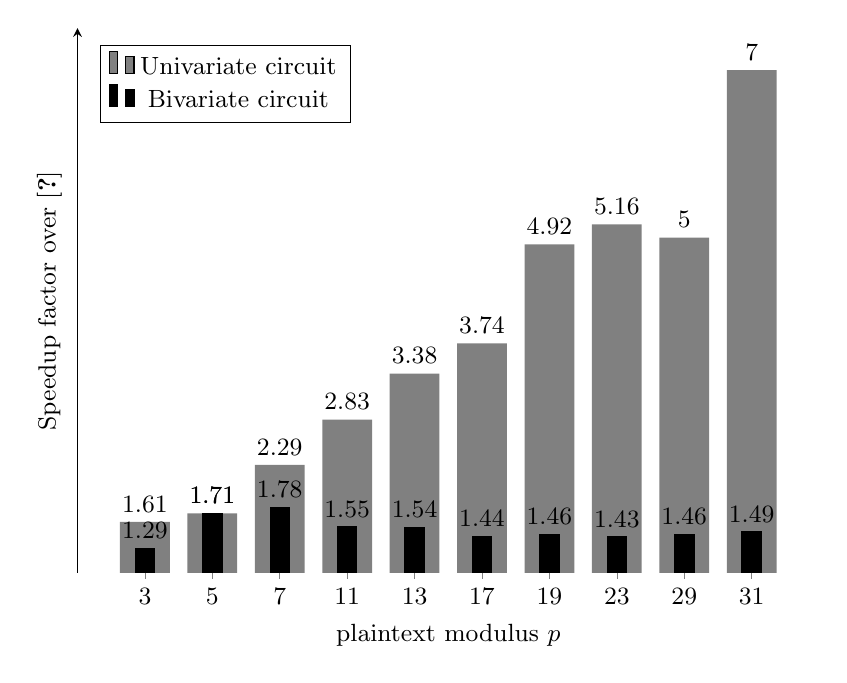
\begin{tikzpicture}
        \begin{axis}[
            width=11.0cm, 
            height=8.5cm, 
            %ymin=0, ymax=240,
            ymin=1, ymax=7.5, 
            xmin=0, xmax=11, 
            axis y line = left, axis x line = bottom,
            x axis line style = {draw=none},
            xtick = {1,2,3,4,5,6,7,8,9,10},
            xticklabels = {3,5,7,11,13,17,19,23,29,31},
            ylabel = {Speedup factor over \cite{TLWRK20}},
            xlabel = {plaintext modulus $p$},
            ytick = \empty,
            legend pos = north west,
            font = \small
            ]
                %\addplot[ybar, ybar legend, fill=white, bar width = 15pt, nodes near coords] coordinates {(1, 90) (2, 36) (3,71) (4,99) (5,54) (6,101) (7,123) (8,232) (9,105) (10,189)};
                %\addlegendentry{\cite{TLWRK20}}
                %\addplot[ybar, ybar legend, fill=gray, bar width = 10pt, nodes near coords] coordinates {(1, 70) (2, 21) (3,40) (4,64) (5,35) (6,70) (7,84) (8,162) (9,72) (10,127)};
                %\addlegendentry{Bivariate circuit}
                %\addplot[ybar, ybar legend, fill=black, bar width = 5pt, nodes near coords] coordinates {(1, 56) (2, 21) (3,31) (4,35) (5,16) (6,27) (7,25) (8,45) (9,22) (10,27)};
                %\addlegendentry{Univariate circuit}
                \addplot[ybar, ybar legend, fill=gray, draw=none, bar width = 18pt, nodes near coords] coordinates {(1, 1.61) (2, 1.71) (3,2.29) (4,2.83) (5,3.38) (6,3.74) (7,4.92) (8,5.16) (9,5) (10,7)};
                \addlegendentry{Univariate circuit}
                \addplot[ybar, ybar legend, fill=black, bar width = 7pt, nodes near coords] coordinates {(1, 1.29) (2, 1.71) (3,1.78) (4,1.55) (5,1.54) (6,1.44) (7,1.46) (8,1.43) (9,1.46) (10,1.49)};
                \addlegendentry{Bivariate circuit}
                
            \end{axis}
    \end{tikzpicture}
    \caption{\textbf{Less-than function via different methods.} The running time speedup factor of our lexicographic order algorithms over the algorithm of Tan et al.~\cite{TLWRK20}. These factors are computed using the data from Table~\ref{table:comparison_circuit_results}.}
    \label{fig:comparison_circuit_results}
\end{figure}
\else
\begin{figure}
    \centering
    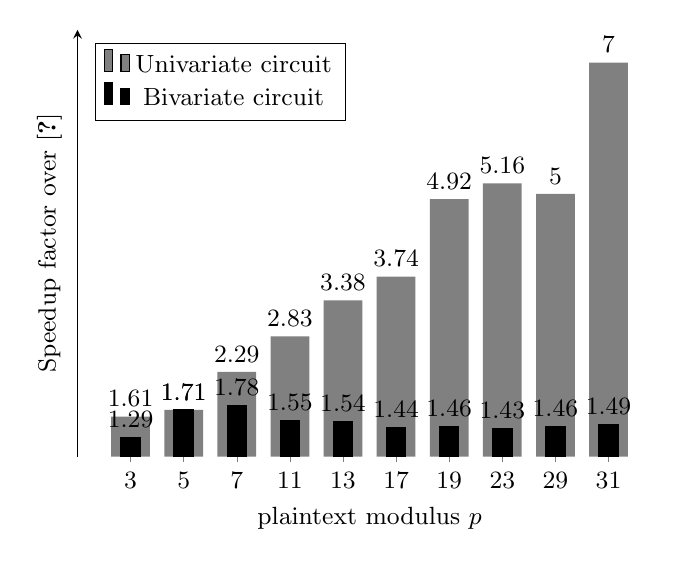
\begin{tikzpicture}
        \begin{axis}[
            width=9.0cm, 
            height=7cm, 
            %ymin=0, ymax=240,
            ymin=1, ymax=7.5, 
            xmin=0, xmax=11, 
            axis y line = left, axis x line = bottom,
            x axis line style = {draw=none},
            xtick = {1,2,3,4,5,6,7,8,9,10},
            xticklabels = {3,5,7,11,13,17,19,23,29,31},
            ylabel = {Speedup factor over \cite{TLWRK20}},
            xlabel = {plaintext modulus $p$},
            ytick = \empty,
            legend pos = north west,
            font = \small
            ]
                %\addplot[ybar, ybar legend, fill=white, bar width = 15pt, nodes near coords] coordinates {(1, 90) (2, 36) (3,71) (4,99) (5,54) (6,101) (7,123) (8,232) (9,105) (10,189)};
                %\addlegendentry{\cite{TLWRK20}}
                %\addplot[ybar, ybar legend, fill=gray, bar width = 10pt, nodes near coords] coordinates {(1, 70) (2, 21) (3,40) (4,64) (5,35) (6,70) (7,84) (8,162) (9,72) (10,127)};
                %\addlegendentry{Bivariate circuit}
                %\addplot[ybar, ybar legend, fill=black, bar width = 5pt, nodes near coords] coordinates {(1, 56) (2, 21) (3,31) (4,35) (5,16) (6,27) (7,25) (8,45) (9,22) (10,27)};
                %\addlegendentry{Univariate circuit}
                \addplot[ybar, ybar legend, fill=gray, draw=none, bar width = 14pt, nodes near coords] coordinates {(1, 1.61) (2, 1.71) (3,2.29) (4,2.83) (5,3.38) (6,3.74) (7,4.92) (8,5.16) (9,5) (10,7)};
                \addlegendentry{Univariate circuit}
                \addplot[ybar, ybar legend, fill=black, bar width = 7pt, nodes near coords] coordinates {(1, 1.29) (2, 1.71) (3,1.78) (4,1.55) (5,1.54) (6,1.44) (7,1.46) (8,1.43) (9,1.46) (10,1.49)};
                \addlegendentry{Bivariate circuit}
                
            \end{axis}
    \end{tikzpicture}
    \caption{\textbf{Less-than function via different methods.} The running time speedup factor of our lexicographic order algorithms over the algorithm of Tan et al.~\cite{TLWRK20}. These factors are computed using the data from Table~\ref{table:comparison_circuit_results}.}
    \label{fig:comparison_circuit_results}
\end{figure}
\fi

As shown in Table~\ref{table:comparison_circuit_results} and Figure~\ref{fig:comparison_circuit_results}, our lexicographic order circuits have a better running time than the prior work of Tan et al.~\cite{TLWRK20} even for small plaintext moduli.
In particular, using our bivariate circuit, the less-than function is 1.71 times faster than with the circuit of Tan et al. on their fastest set of parameters ($(p,d,l) = (5,7,4)$).
The best running time per integer was achieved by our univariate circuit, which outperforms any bivariate circuit for any $p > 5$ at the cost of larger encryption parameters.
As shown in Figure~\ref{fig:comparison_circuit_results}, the speedup factor of the lexicographic order with the univariate circuit over~\cite{TLWRK20} is increasing with the plaintext modulus.
This trend is perturbed when $p=23$ and $29$ because the structure of the related slot permutation groups introduces additional computational overhead and ciphertext noise, thus leading to larger encryption parameters. 

Table~\ref{table:univariate_circuit_results} shows that for $p=131$, the univariate circuit takes only 11 milliseconds to compare two 64-bit integers, which is more than 3 times faster than the best running time achieved by the circuit of Tan et al.

\ifeprint
\begin{table}[h!]
  \centering
  \begin{tabular*}{.9\textwidth}{@{\extracolsep{\fill}} p{0.3cm} p{0.7cm} p{0.8cm} p{2.0cm} p{2.5cm} p{2.5cm}}
    \toprule
    $N$     & $\log_2 q$    & \#Trials  & Average total time, s & Amortized time per integer, ms & Amortized time per integer, ms~\cite{CDSS15} \\
    \midrule
    \multicolumn{6}{l}{8-bit integers ($d=2$, $l=1$, $k=9352$)} \\
    \cmidrule(lr){1-6}
    4       & 589     & 32        & 186.28       & 20    & 140 \\
    8       & 599     & 20        & 867.46       & 93    & 690 \\
    16      & 599     & 20        & 3652.23      & 391   & 3140\\
    32      & 599     & 20        & 14769.23     & 1579  & 13900 \\
    64      & 604     & 10        & 60351.02     & 6453  & 60000 \\
    \midrule
    \multicolumn{6}{l}{32-bit integers ($d=3$, $l=2$, $k=4676$)} \\
    \cmidrule(lr){1-6}
    4       & 659     & 20        & 299.17       & 64    & 200 \\
    8       & 671     & 20        & 1356.19      & 290   & 944 \\
    16      & 671     & 20        & 5700.12      & 1219  & 4280 \\
    32      & 684     & 20        & 23017.03     & 4922  & 18600 \\
    64      & 684     & 10        & 89972.27     & 19241 & 49700 \\
    \bottomrule
  \end{tabular*}
  \caption{\textbf{Sorting.} The running time needed to sort $N$ 8-bit or 32-bit integers with $p=167$, $m=28057$ and $n=28056$. The minimal security level is 92 bits according to the LWE estimator~\cite{lwe_estimator}. Note that the amortized timing per integer from~\cite{CDSS15} is obtained with the LTV scheme~\cite{STOC:LopTroVai12}, which was attacked by Albrecht et al.~\cite{C:AlbBaiDuc16}.}
  \label{table:sorting_circuit_results}
\end{table}
\else
\begin{table}[h]
  \centering
  \begin{tabular*}{.45\textwidth}{ p{0.3cm} p{0.7cm} p{0.8cm} p{1cm} p{1.3cm} p{1.5cm}}
    \toprule
    $N$     & $\log_2 q$    & \#Trials  & Average total time, s & Amortized time per integer, ms & Amortized time per integer, ms~\cite{CDSS15} \\
    \midrule
    \multicolumn{6}{l}{8-bit integers ($d=2$, $l=1$, $k=9352$)} \\
    \cmidrule(lr){1-6}
    4       & 589     & 32        & 186.28       & 20    & 140 \\
    8       & 599     & 20        & 867.46       & 93    & 690 \\
    16      & 599     & 20        & 3652.23      & 391   & 3140\\
    32      & 599     & 20        & 14769.23     & 1579  & 13900 \\
    64      & 604     & 10        & 60351.02     & 6453  & 60000 \\
    \midrule
    \multicolumn{6}{l}{32-bit integers ($d=3$, $l=2$, $k=4676$)} \\
    \cmidrule(lr){1-6}
    4       & 659     & 20        & 299.17       & 64    & 200 \\
    8       & 671     & 20        & 1356.19      & 290   & 944 \\
    16      & 671     & 20        & 5700.12      & 1219  & 4280 \\
    32      & 684     & 20        & 23017.03     & 4922  & 18600 \\
    64      & 684     & 10        & 89972.27     & 19241 & 49700 \\
    \bottomrule
  \end{tabular*}
  \caption{\textbf{Sorting.} The running time needed to sort $N$ 8-bit or 32-bit integers with $p=167$, $m=28057$ and $n=28056$. The minimal security level is 92 bits according to the LWE estimator~\cite{lwe_estimator}. Note that the amortized timing per integer from~\cite{CDSS15} is obtained with the LTV scheme~\cite{STOC:LopTroVai12}, which was attacked by Albrecht et al.~\cite{C:AlbBaiDuc16}.}
  \label{table:sorting_circuit_results}
\end{table}
\fi

Table~\ref{table:sorting_circuit_results} illustrates that our homomorphic sorting implementation achieves the best running time in the existing literature.
Note that the best result~\cite{CDSS15} in this area is based on an SHE scheme that was successfully attacked by Albrecht et al.~\cite{C:AlbBaiDuc16}.
Hence, this result is hard to compare directly to our work.

\ifeprint
\begin{table}[h!]
  \centering
  \begin{tabular*}{.8\textwidth}{@{\extracolsep{\fill}} p{0.8cm} p{0.8cm} p{1.0cm} p{1.5cm} p{2.0cm} p{2.5cm}}
    \toprule
    $N$     & $T$   & $\log_2 q$    & \#Trials  & Average total time, s    & Amortized time per integer, ms \\
    \midrule
    \multicolumn{6}{l}{8-bit integers ($d=3$, $l=1$, $k=5220$)} \\
    \cmidrule(lr){1-6}
    2       & 1     & 232           & 20        & 12.35     & 2.37 \\
    4       & 2     & 406           & 20        & 50.55     & 9.68 \\
    8       & 3     & 579           & 20        & 151.75    & 29.07 \\
    16      & 4     & 766           & 20        & 386.87    & 74.11 \\
    32      & 3     & 825           & 20        & 883.68    & 169.29 \\
    64      & 3     & 854           & 20        & 2111.56   & 404.51 \\
    \midrule
    \multicolumn{6}{l}{32-bit integers ($d=6$, $l=2$, $k=2610$)} \\
    \cmidrule(lr){1-6}
    2       & 1     & 406           & 20        & 37.71     & 14.54 \\
    4       & 2     & 753           & 20        & 157.80    & 60.46 \\
    8       & 1     & 825           & 20        & 506.24    & 193.96 \\
    16      & 1     & 839           & 20        & 1694.15   & 649.10 \\
    32      & 1     & 854           & 20        & 6440.27   & 2467.54 \\
    64      & 1     & 884           & 20        & 24986.04  & 9573.20 \\
    \bottomrule
  \end{tabular*}
  \caption{\textbf{Array minimum.} The running time needed to find the minimum of $N$ 8-bit or 32-bit integers with $p=17$, $m=41761$ and $n=41760$. The parameter $T$ denotes the number of the tournament method stages. The minimal security level is 121 bits according to the LWE estimator~\cite{lwe_estimator}.}
  \label{table:minimum_circuit_results}
\end{table}
\else
\begin{table}[h]
  \centering
  \begin{tabular*}{.45\textwidth}{ p{0.2cm} p{0.2cm} p{0.8cm} p{0.9cm} p{1.5cm} p{2.0cm}}
    \toprule
    $N$     & $T$   & $\log_2 q$    & \#Trials  & Average total time, s    & Amortized time per integer, ms \\
    \midrule
    \multicolumn{6}{l}{8-bit integers ($d=3$, $l=1$, $k=5220$)} \\
    \cmidrule(lr){1-6}
    2       & 1     & 232           & 20        & 12.35     & 2.37 \\
    4       & 2     & 406           & 20        & 50.55     & 9.68 \\
    8       & 3     & 579           & 20        & 151.75    & 29.07 \\
    16      & 4     & 766           & 20        & 386.87    & 74.11 \\
    32      & 3     & 825           & 20        & 883.68    & 169.29 \\
    64      & 3     & 854           & 20        & 2111.56   & 404.51 \\
    \midrule
    \multicolumn{6}{l}{32-bit integers ($d=6$, $l=2$, $k=2610$)} \\
    \cmidrule(lr){1-6}
    2       & 1     & 406           & 20        & 37.71     & 14.54 \\
    4       & 2     & 753           & 20        & 157.80    & 60.46 \\
    8       & 1     & 825           & 20        & 506.24    & 193.96 \\
    16      & 1     & 839           & 20        & 1694.15   & 649.10 \\
    32      & 1     & 854           & 20        & 6440.27   & 2467.54 \\
    64      & 1     & 884           & 20        & 24986.04  & 9573.20 \\
    \bottomrule
  \end{tabular*}
  \caption{\textbf{Array minimum.} The running time needed to find the minimum of $N$ 8-bit or 32-bit integers with $p=17$, $m=41761$ and $n=41760$. The parameter $T$ denotes the number of the tournament method stages. The minimal security level is 121 bits according to the LWE estimator~\cite{lwe_estimator}.}
  \label{table:minimum_circuit_results}
\end{table}
\fi

The existing literature on homomorphic array minimum/maximum algorithms~\cite{TMP15,PoPETS:SFR20} is based on the techniques described in Section~\ref{sec:min/max}.
Hence, our improvement of comparison circuits automatically results in a better performance over these works.  
For example, Togan et al.~\cite{TMP15} needed 346.9 seconds to find maximal elements of 960 arrays of 16 8-bit integers, which is 361 milliseconds per array.
Our work can perform this task in 74 milliseconds, see Table~\ref{table:minimum_circuit_results}.
To find the minimum of 64 32-bit integers, our array minimum algorithm requires about 9.5 seconds.

\subsection{Comparison to other HE schemes}
    As mentioned in the introduction, there are three types of HE schemes suitable in different use cases including TFHE, CKKS and BGV/BFV.
    Our algorithms are designed for BGV/BFV, which support SIMD packing and are the most efficient FHE schemes for exact computation in arithmetic circuits.
    However, the amortized running time per data value of our comparison algorithms is comparable to efficient FHE schemes for binary circuits (TFHE) and HE supporting approximate arithmetic over complex numbers (CKKS). 

    In Table~\ref{table:other_he_schemes}, our implementation of the less-than function is compared to the implementations of this function in TFHE \cite{AC:CGGI17,JC:CGGI20} and CKKS \cite{EPRINT:CheKimKim19}.

    Chilloti et al.~\cite{AC:CGGI17,JC:CGGI20} constructed a deterministic weighted automata that can compute the maximum function using the TFHE scheme.
    The same automata can compute the less-than function without any performance loss. 
    In this case, the running time of the less-than function of two $b$-bit integers takes $170 b$ microseconds on a hardware similar to ours and with the encryption parameters supporting at least 152 bits of security.
    This security level might be lowered by a recent attack of Espitau et al.~\cite{EPRINT:EJK20}.
    Note that this running time is achieved in the leveled mode of TFHE, i.e. without bootstrapping.
    Unfortunately, we could not manage to run the code of this implementation on our machine.

    Cheon et al. \cite{EPRINT:CheKimKim19} designed a polynomial approximation of the less-than function over real numbers.
    Since the precision of this approximation depends on the ciphertext noise which cannot be reduced in CKKS, only a few consecutive comparisons are possible to perform correctly unlike in TFHE and BGV/BFV.
    Nevertheless, the number of SIMD slots in CKKS is always half of the ring dimension ($n/2$), which significantly reduces the amortized running time per value.

    We ran the comparison method of Cheon et al. on our machine with multi-threading turned off. 
    Since the implementation in~\cite{EPRINT:CheKimKim19} uses parallelization with 8 cores, our running time of this method presented in Table~\ref{table:other_he_schemes} is significantly larger than in~\cite{EPRINT:CheKimKim19}.
    The encryption parameters of the CKKS scheme are set to support a security level of at least 128 bits.

    Our implementation runs with $p=131$, $m=17293$ ($n=17292$), which corresponds to 5764 integers of 8-16 bits or 2882 20-bit integers encoded into one ciphertext.
    The encryption parameters corresponds to a security level of at least 126 bits.

    \ifeprint
    \begin{table}[h!]
      \centering
      \begin{tabular*}{.8\textwidth}{ p{1.8cm} p{3.1cm} p{2.0cm} p{2.3cm}}
        \toprule
        Bit length  & FHE scheme & Total time, s    & Amortized time per integer, ms \\
        \midrule
        \multirow{3}{*}{8}  & TFHE              & 0.001*     & 1.36* \\
                            & CKKS              & 89.61     & 1.37 \\
                            & BGV(this paper)   & 7.09      & 1.23 \\
        \midrule
        \multirow{3}{*}{12}  & TFHE             & 0.002*     & 2.04* \\
                             & CKKS             & 127.54    & 1.95 \\
                             & BGV(this paper)  & 7.09      & 1.23 \\
        \midrule
        \multirow{3}{*}{16}  & TFHE            & 0.003*     & 2.72* \\
                             & CKKS            & 296.96     & 4.53 \\
                             & BGV(this paper)  & 12.11      & 2.10 \\
        \midrule
        \multirow{3}{*}{20}  & TFHE            & 0.003*      & 3.4* \\
                             & CKKS            & 373.76     & 5.70 \\
                             & BGV(this paper)   & 8.66     &  3.01\\ 
        \bottomrule
      \end{tabular*}
      \caption{\textbf{Comparison with other HE schemes.} Total and amortized running time of the less-than function implemented with different HE schemes including TFHE, CKKS and BGV. Note that TFHE does not support SIMD packing, which implies that the total and amortized running time of this scheme are the same. The encryption parameters of each scheme are set to support the following security levels: 152 bits for TFHE (might be smaller due to~\cite{EPRINT:EJK20}), 128 bits for CKKS and 126 bits for BGV.
      \newline *TFHE timings are estimated from~\cite{JC:CGGI20}.}
      \label{table:other_he_schemes}
    \end{table}
    \else
    \begin{table}[h]
      \centering
      \begin{tabular*}{.45\textwidth}{ p{1.2cm} p{2.1cm} p{1.0cm} p{2cm}}
        \toprule
        Bit length  & FHE scheme & Total time, s    & Amortized time per integer, ms \\
        \midrule
        \multirow{3}{*}{8}  & TFHE              & 0.001*     & 1.36* \\
                            & CKKS              & 89.61     & 1.37 \\
                            & BGV(this paper)   & 7.09      & 1.23 \\
        \midrule
        \multirow{3}{*}{12}  & TFHE             & 0.002*     & 2.04* \\
                             & CKKS             & 127.54    & 1.95 \\
                             & BGV(this paper)  & 7.09      & 1.23 \\
        \midrule
        \multirow{3}{*}{16}  & TFHE            & 0.003*     & 2.72* \\
                             & CKKS            & 296.96     & 4.53 \\
                             & BGV(this paper)  & 12.11      & 2.10 \\
        \midrule
        \multirow{3}{*}{20}  & TFHE            & 0.003*      & 3.4* \\
                             & CKKS            & 373.76     & 5.70 \\
                             & BGV(this paper)   & 8.66     &  3.01\\ 
        \bottomrule
      \end{tabular*}
      \caption{\textbf{Comparison with other HE schemes.} Total and amortized running time of the less-than function implemented with different HE schemes including TFHE, CKKS and BGV. Note that TFHE does not support SIMD packing, which implies that the total and amortized running time of this scheme are the same. The encryption parameters of each scheme are set to support the following security levels: 152 bits for TFHE (might be smaller due to~\cite{EPRINT:EJK20}), 128 bits for CKKS and 126 bits for BGV.
      \newline *TFHE timings are estimated from~\cite{JC:CGGI20}.}
      \label{table:other_he_schemes}
    \end{table}
    \fi
    
    As shown in Table~\ref{table:other_he_schemes}, our algorithm for the less-than function demonstrates a similar performance as the TFHE-based implementation and is up to 2 times faster than the CKKS-based work.
    This means that in use cases that involve arithmetic and non-arithmetic functions (e.g. artificial neural networks) one might resort to only an HE scheme supporting exact arithmetic circuits (i.e. BGV/BFV) instead of combining it with an HE scheme efficient for a non-arithmetic part of the computation (i.e. TFHE).
    
%%% Local Variables:
%%% mode: latex
%%% TeX-master: "main_pets"
%%% End:

% \section{Old ideas}
% The homomorphic circuit for $\LT_{\F_\fieldcard}(x,y)$ is presented in Algorithm~\ref{alg:basic_less_than_circuit}.
Unlike the prior works (\todo{cite}) that evaluate this circuit as a multivariate polynomial, we exploit its representation in~(\ref{eq:less_than_function}) to parallelize computations in the SIMD manner. 
\begin{algorithm}[t]
  \KwIn{
  $\ct_x$ -- a ciphertext encrypting $x \in \F_\fieldcard$ in the first SIMD slot and $0$ in other slots,
  $\ct_y$ -- a ciphertext encrypting $y \in \F_\fieldcard$ in the first SIMD slot and $0$ in other slots,
  $\S = \{a_0,a_1,\dots,a_{\fieldcard-1}\}$ -- a complete set of representatives of $\F_\fieldcard$.
  }
  \KwOut{$\ct$ -- a ciphertext encrypting $1$ in the first SIMD slot if $x < y$, otherwise $0$. Other slots contain $0$.}
  $\ct_1 \leftarrow \Replicate(\ct_x, \fieldcard - 1)$//\todo{Define replicate}\\
  $\ct_2 \leftarrow \Replicate(\ct_y, \fieldcard - 1)$\\
  $\pt_1 \leftarrow \pt(a_0, a_1, \dots, a_{\fieldcard-2})$//\todo{define this operation}\\
  $\pt_2 \leftarrow \pt(a_1, a_2, \dots, a_{\fieldcard-1})$\\
  $\ct_1 \leftarrow \ct_1 - \pt_1$//\todo{define operations between ciphertexts and plaintexts}\\
  $\ct_2 \leftarrow \ct_2 - \pt_2$\\
  $\ct_1 \leftarrow \ct_1^{\fieldcard-1}$//$\princhar_\fieldcard(x-a)$, \todo{define this operation}\\
  $\ct_2 \leftarrow \ct_2^{\fieldcard-1}$//$\princhar_\fieldcard(y-b)$\\
  $\ct_1 \leftarrow 1 - \ct_1$// define operations between constants and ciphertexts\\
  $\ct_2 \leftarrow 1 - \ct_2$\\
  $k \leftarrow 1$// compute all running sums $\sum_{b \in \S, a < b} (1-\princhar_\fieldcard(x - b))$ \\
  \While{$k < \fieldcard-1$}{
    $\ct_{tmp} \leftarrow \Shift(\ct_2, k)$//\todo{define shift}\\
    $\ct_2 \leftarrow \ct_2 + \ct_{tmp}$\\
    $k \leftarrow 2k$\\
  }
  $\ct \leftarrow \ct_1 \cdot \ct_2$\\
  $k \leftarrow 1$\\
  \While{$k < \fieldcard-1$}{
    $\ct_{tmp} \leftarrow \Shift(\ct, k)$\\
    $\ct \leftarrow \ct + \ct_{tmp}$\\
    $k \leftarrow 2k$\\
  }
  $\ct \leftarrow \Select(\ct, \{1\})$//\todo{define select}\\
  \textbf{Return} $\ct$.
  \caption{Homomorphic circuit of $\LT_{\F_\fieldcard}$.}\label{alg:basic_less_than_circuit}
\end{algorithm}
\todo{Make a separate algorithm for running sums (while circuit above)}
\todo{Write down the complexity of Algorithm~\ref{alg:basic_less_than_circuit}, compare with prior works}

Here are potential cyclotomic polynomials to use for a failure probability smaller $\varepsilon < 2^{-32}$.

\begin{table}
  \setlength{\tabcolsep}{1em}
  \centering
  \begin{tabular}{||ccc||cccccc||}
    \hline
    $~m~$ & $~n~$ & $~\delta_\mathcal{R}~$ & $~p~$ & $~d~$ & depth & $~\ell~$ & $~s~$ & $~\varepsilon~$ \\
    \hline
    $22,383$ & $14,904$ & $5n$ & $5$  & $18$ & $8$ & $828$  & $1$ &  $2^{-41.7}$ \\
    $25,623$ & $15,552$ & $118n$ & $2$ & $36$ & $7$ & $432$ & $2$ & $2^{-36.0}$ \\
    $31,132$ & $15,120$ & $85n$ & $7$ & $12$ & $8$ & $1,260$ & $2$ & $2^{-33.6}$ \\
    $31,726$ & $15,288$ & $57n$ & $3$ & $28$ & $7$ & $546$ & $1$ & $2^{-44.3}$ \\
    $35,552$ & $16,000$ & $21n$ & $17$ & $10$ & $9$ & $1,600$ & $3$ & $2^{-40.8}$ \\
    \hline
    $31,697$ & $30,576$ & $57n$ & $3$ & $28$ & $7$ & $1,092$ & $1$ & $2^{-44.3}$ \\
    $48,771$ & $32,508$ & $5n$ & $2$ & $42$ & $7$ & $774$ & $1$ & $2^{-42.0}$ \\
    $57,368$ & $28,000$ & $141n$ & $17$ & $10$ & $9$ & $2,800$ & $3$ & $2^{-40.8}$ \\
    $72,400$ & $28,800$ & $9n$ & $7$ & $12$ & $8$ & $2,400$ & $3$ & $2^{-33.6}$ \\
    $93,006$ & $30,996$ & $5n$ & $5$ & $18$ & $8$ & $1,722$ & $1$ & $2^{-41.7}$ \\
    \hline
                                                   
  \end{tabular}
  \caption{Potential parameters}
  \label{tab:params}
\end{table}

\begin{itemize}
\item $m$: cyclotomic order;
\item $n$: degree of the cyclotomic;
\item $\delta_\mathcal{R}$: expansion factor (upper-bound);
\item $p$: plaintext modulus;
\item $d$: degree of the factors of $\phi_m$ modulo $p$;
\item depth: $\lceil \log_2(p-1) \rceil + \lceil \log_2(d)\rceil + 1$;
\item $\ell$: number of factors of of $\phi_m$ modulo $p$;
\item $s$: number of generators for $(\Z/m\Z)^\times/<p>$;
\item $\varepsilon$: approximative probability of failure for one equality check.
\end{itemize}

\remove{
\subsection{Min/Max function on vectors}

  \begin{align*}
    \min_\S(\vx,\vy) = \vx \cdot \LT_\S(\vx,\vy) + \vy \cdot (1 - \LT_\S(\vx,\vy)).
  \end{align*}

  \begin{align*}
    \LT_{\F_\fieldcard}(\vx, \vy) = \sum_{i=0}^{\ell-2} \LT_{\F_\fieldcard}(x_{i}, y_{i}) \prod_{j=i+1}^{\ell-1} \EQ_{\F_\fieldcard}(x_{j}, y_{j}) + \LT_{\F_\fieldcard}(x_{\ell-1}, y_{\ell-1}).
  \end{align*}

  \begin{align*}
    (x-y) \cdot \EQ_{\F_p}(x,y) = 0
  \end{align*}
  
  \begin{align*}
    \min_\S(\vx,\vy)_k &= x_k \cdot \LT_\S(\vx,\vy) + y_k \cdot (1 - \LT_\S(\vx,\vy)) \\
    &= y_k + (x_k - y_k) \cdot \LT_\S(\vx,\vy)) \\
    &= y_k + (x_k - y_k) \cdot \left(\sum_{i=0}^{\ell-1} \LT_{\F_\fieldcard}(x_{i}, y_{i}) \prod_{j=i+1}^{\ell-1} \EQ_{\F_\fieldcard}(x_{j}, y_{j})\right) \\
    &= y_k + (x_k - y_k) \cdot \left(\sum_{i=0}^{k-1} \LT_{\F_\fieldcard}(x_{i}, y_{i}) \prod_{j=i+1}^{\ell-1} \EQ_{\F_\fieldcard}(x_{j}, y_{j})\right) \\
    &+ (x_k - y_k) \cdot \left(\sum_{i=k}^{\ell-1} \LT_{\F_\fieldcard}(x_{i}, y_{i}) \prod_{j=i+1}^{\ell-1} \EQ_{\F_\fieldcard}(x_{j}, y_{j})\right) \\
    &= y_k + (x_k - y_k) \cdot \left(\sum_{i=k}^{\ell-1} \LT_{\F_\fieldcard}(x_{i}, y_{i}) \prod_{j=i+1}^{\ell-1} \EQ_{\F_\fieldcard}(x_{j}, y_{j})\right)
  \end{align*}
  }



\bibliographystyle{plain}
\bibliography{abbrev3,biblio}


\end{document}

%%% Local Variables:
%%% mode: latex
%%% TeX-master: t
%%% End:
